% =====================================================================
%  Tomato Doctor - IEEE conference-format paper
%  Compile with XeLaTeX or Tectonic (needs the Tamil font in ./fonts):
%      tectonic main.tex        or        latexmk -xelatex main.tex
%  Every number in this paper is produced by scripts/experiments.py
%  (raw results in ./results) and every chart by make_figures.py.
% =====================================================================
\documentclass[conference]{IEEEtran}
\IEEEoverridecommandlockouts

\usepackage{fontspec}
\usepackage{unicode-math}
\setmainfont{texgyretermes}[Extension=.otf, UprightFont=*-regular, BoldFont=*-bold, ItalicFont=*-italic, BoldItalicFont=*-bolditalic]
\setmathfont{texgyretermes-math.otf}
\setsansfont{texgyreheros}[Extension=.otf, UprightFont=*-regular, BoldFont=*-bold, ItalicFont=*-italic, BoldItalicFont=*-bolditalic]
\setmonofont{texgyrecursor}[Extension=.otf, UprightFont=*-regular, BoldFont=*-bold, ItalicFont=*-italic, BoldItalicFont=*-bolditalic, Scale=0.95]
\newfontfamily\tamilfont[Path=./fonts/, Script=Tamil, BoldFont=NotoSansTamil-Bold.ttf, Scale=0.92]{NotoSansTamil-Regular.ttf}
\newcommand{\ta}[1]{{\tamilfont #1}}

\usepackage{amsmath}
\usepackage{booktabs,multirow,array}
\usepackage{graphicx}
\usepackage[caption=false,font=footnotesize]{subfig}
\usepackage{algorithm}
\usepackage{algpseudocode}
\usepackage{xcolor}
\usepackage{tikz}
\usetikzlibrary{positioning,arrows.meta,shapes,fit,calc,backgrounds}
\usepackage{cite}
\usepackage{xurl}
\usepackage[hidelinks]{hyperref}

\newcommand{\unk}{\textsc{unknown}}
\newcommand{\EIG}{\mathrm{EIG}}
\renewcommand{\algorithmicrequire}{\textbf{Input:}}
\renewcommand{\algorithmicensure}{\textbf{Output:}}

\begin{document}

\title{Tomato Doctor: A Tamil-First Conversational Crop-Disease Diagnosis System on a Probabilistic Knowledge Graph with Information-Gain Questioning and Weather-Aware Advisory}

\author{%
\IEEEauthorblockN{Author Name\IEEEauthorrefmark{1}, Author Name\IEEEauthorrefmark{1}, Author Name\IEEEauthorrefmark{1}, and Guide Name\IEEEauthorrefmark{2}}
\IEEEauthorblockA{\IEEEauthorrefmark{1}Department of Computer Science and Engineering, Institution Name, City, India}
\IEEEauthorblockA{\IEEEauthorrefmark{2}Department, Institution Name, City, India\\
Email: \{author1, author2\}@institution.edu}
}

\maketitle

% =====================================================================
\begin{abstract}
Smallholder tomato growers describe crop problems in colloquial, mixed-script language, often without a usable photograph, while most digital diagnosis tools are image classifiers trained on laboratory photographs. We present \emph{Tomato Doctor}, a Tamil-first diagnosis system that reasons over a probabilistic knowledge graph (KG) of 17 diseases and pests, 45 observable symptoms, 247 Tamil, English and Tanglish lay-terms and 30 cited treatments. A concept-level language layer with Tamil stem matching, negation scope and IDF-weighted phrase coverage turns free text into reliability-weighted symptom evidence; a Bayesian engine with an explicit \unk{} hypothesis fuses that evidence with a calibrated leaf-photo classifier and a weather-driven prior, and asks the follow-up question with the highest expected information gain. Confirmed outcomes update Beta-distributed KG edge weights, and an advisory layer turns local hourly weather into spray windows, resistance-aware rotation and a dated schedule. On 85 held-out farmer descriptions with simulated noisy dialogues, top-1 accuracy rises from 63.5\% (95\% CI 52.9--74.1) for the fuzzy-matching prototype to 96.8\% (94.5--98.5), while confidently wrong answers fall from 10.6\% to 1.2\%; information-gain questioning needs 2.1 questions on average, 37\% fewer than a weight-variance heuristic at equal accuracy. Under field-like photo degradation the classifier alone drops to 36.4\%, whereas fusing the same photo with the dialogue recovers 67.8\%. Starting from a deliberately corrupted graph, confirmation-driven learning raises accuracy from 81.2\% to 93.6\% over 1,500 simulated consultations and nearly halves the mean edge-weight error, whereas the prototype's update rule increases it. A request costs 3.7\,ms on a laptop CPU.
\end{abstract}

\begin{IEEEkeywords}
Knowledge graphs, plant disease diagnosis, Bayesian inference, expected information gain, low-resource languages, Tamil, decision support systems, precision agriculture.
\end{IEEEkeywords}

% =====================================================================
\section{Introduction}

Early, correct identification of a crop disease decides whether a farmer sprays the right product at the right time or loses part of a harvest. Deep convolutional networks recognise diseases in curated leaf photographs with high accuracy~\cite{mohanty2016,ferentinos2018}, yet their accuracy falls sharply on images taken in the field, with cluttered backgrounds, multiple symptoms and variable lighting~\cite{ferentinos2018,barbedo2018}. Moreover, an image-only tool assumes that the farmer can and will produce a clear photograph, and it cannot use the most informative signal the farmer already has: what they saw, said in their own words.

For Tamil-speaking growers that description is colloquial, agglutinative and frequently code-mixed with English or written in Latin script (``Tanglish''), e.g.\ \ta{இலையில் வெள்ளை தூள் போல இருக்கு} (``white dust-like stuff on the leaf''). Such descriptions are also genuinely ambiguous: ``white dust'' fits both powdery mildew and a whitefly infestation, two problems with entirely different treatments. A useful system must therefore (i) understand informal multilingual text robustly, (ii) recognise when the evidence is insufficient and ask the \emph{one} question that best separates the remaining candidates, (iii) remain usable when the photograph is poor, (iv) adapt treatment advice to the local weather that determines both disease pressure and whether a spray will wash off, and (v) improve as farmers confirm or correct its answers.

A first prototype of this project stored diseases, symptoms, Tamil lay-terms and treatments in a Neo4j graph, matched farmer text to lay-terms with whole-phrase fuzzy matching and summed edge weights to rank diseases. Analysing it revealed failure modes that motivate this work: shared filler words caused spurious matches, negation was ignored, answers to follow-up questions did not influence the ranking, and a single rejection decayed edge weights for all future users.

This paper makes the following contributions:
\begin{enumerate}
  \item A \textbf{probabilistic agricultural KG} whose symptom and lay-term edges are Beta posteriors, with cited treatments annotated by mode of action, FRAC/IRAC resistance group, rain-fastness, heat limit and dose (Section~\ref{sec:kg}).
  \item A \textbf{concept-level multilingual symptom matcher} for Tamil, English and Tanglish with stem matching, negation scope and IDF-weighted coverage, plus an LLM front end that is \emph{constrained to the KG's vocabulary} for speech (Section~\ref{sec:nlu}).
  \item A \textbf{Bayesian diagnosis engine} with reliability-weighted asymmetric evidence, an explicit \unk{} hypothesis, tempered photo-likelihood fusion and cost-aware expected-information-gain questioning (Section~\ref{sec:inference}).
  \item A \textbf{weather- and location-aware advisory layer}: published disease-forecast models (Hutton criteria, TOM-CAST) as a data-driven prior, spray-window planning, severity-adaptive and resistance-aware treatment plans, and community outbreak alerts (Section~\ref{sec:advisory}).
  \item \textbf{Confirmation-driven online learning} that only learns from verified outcomes (Section~\ref{sec:learning}), and an evaluation with ablations, a photo-robustness study, a learning simulation and a live weather case study (Section~\ref{sec:eval}).
\end{enumerate}

% =====================================================================
\section{Related Work}

\subsection{Image-based plant disease recognition}
The PlantVillage collection~\cite{hughes2015} enabled convolutional models that reach high accuracy on held-out laboratory images~\cite{mohanty2016,ferentinos2018}. The same studies, and a dedicated analysis of influencing factors~\cite{barbedo2018}, report substantial degradation under field conditions caused by background, illumination, symptom variability and co-occurring disorders. We use such a classifier as one source of evidence and quantify how fusion with dialogue changes its behaviour under degradation.

\subsection{Probabilistic diagnosis and question selection}
Normative expert systems such as Pathfinder~\cite{heckerman1992} and the probabilistic reformulation of INTERNIST-1/QMR~\cite{shwe1991} represent diagnosis as Bayesian inference over findings; Pathfinder additionally chooses the next finding to observe by its expected value of information, and the expected information gain of an experiment goes back to Lindley~\cite{lindley1956}. We adapt this line of work to an agricultural KG whose findings arrive through noisy language understanding rather than structured entry, and model that noise explicitly.

\subsection{Agricultural knowledge graphs and conversational agents}
Knowledge graphs organise entities and typed relations for retrieval and reasoning~\cite{hogan2021}. AgriKG~\cite{chen2019agrikg} extracts agricultural entities from web text into a graph for entity retrieval and question answering. FarmChat~\cite{jain2018farmchat} showed that a speech-based conversational agent built from Kisan Call Centre logs can meet the information needs of low-literate farmers in India. Our system differs in that the KG is \emph{probabilistic} and drives an adaptive diagnostic dialogue, and in that weights change with verified field outcomes.

\subsection{Language technology for Indian languages}
IndicNLPSuite~\cite{kakwani2020} provides corpora and multilingual models for Indian languages, and large-scale weakly supervised speech recognition~\cite{radford2023whisper} and multimodal large language models~\cite{gemini2023} now transcribe Tamil speech. Colloquial agricultural symptom descriptions remain a low-resource domain, which motivates our lightweight, inspectable concept lexicon and the use of an LLM only as a constrained entity linker.

\subsection{Weather-driven disease forecasting}
Disease forecasters convert weather into infection risk: FAST~\cite{madden1978} and its TOM-CAST derivative accumulate daily disease-severity values (DSVs) from leaf wetness and temperature for early blight~\cite{frost2015}; the Smith Period and the more sensitive Hutton Criteria flag late-blight risk from consecutive warm, humid days~\cite{ahdb_hutton}. We use these models, together with rules derived from a tomato disease dataset~\cite{jagtap2025}, as a prior for diagnosis and as an early warning.

% =====================================================================
\section{System Overview}
\label{sec:overview}

Fig.~\ref{fig:arch} shows the architecture. A Tamil-first progressive web application collects free text, voice, a leaf photograph, location, and optional tapped symptoms, severity, extent and previously sprayed products. Four extractors turn these inputs into evidence: the concept matcher (Section~\ref{sec:nlu}), an LLM entity linker for speech, a leaf-photo classifier, and a field-context service that fetches hourly weather and nearby outbreak reports. The reasoning core maintains a posterior over diseases (Section~\ref{sec:inference}); while no hypothesis is confident it asks the most informative question, otherwise it returns a diagnosis with an evidence-level explanation and a weather-aware treatment plan (Section~\ref{sec:advisory}). Farmer confirmations and expert curation close the loop (Section~\ref{sec:learning}).

\begin{figure*}[t]
  \centering
  \resizebox{\textwidth}{!}{% System architecture (Fig. 1)
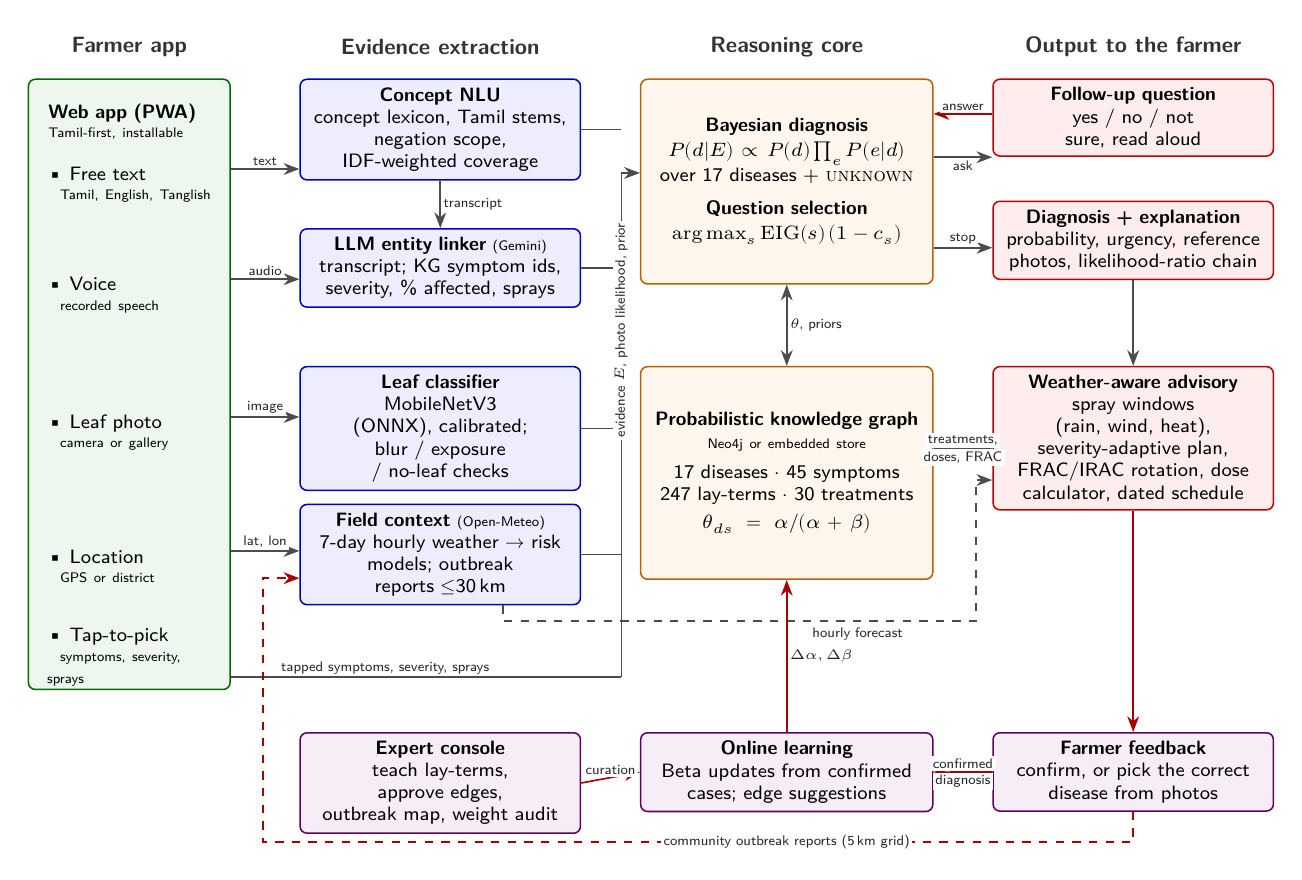
\begin{tikzpicture}[
  font=\sffamily\scriptsize, >=Stealth,
  box/.style={draw=#1!75!black, fill=#1!7, rounded corners=2.5pt, align=center, inner sep=3pt, line width=0.55pt, text width=3.35cm},
  hdr/.style={font=\sffamily\footnotesize\bfseries, align=center, text=black!80},
  flow/.style={->, line width=0.6pt, draw=black!70},
  back/.style={->, line width=0.6pt, draw=red!65!black},
  lbl/.style={font=\sffamily\tiny, fill=white, inner sep=0.9pt, align=center, text=black!85},
]
% ---------------- headers
\node[hdr] at (1.35, 0.55) {Farmer app};
\node[hdr] at (5.3, 0.55) {Evidence extraction};
\node[hdr] at (9.7, 0.55) {Reasoning core};
\node[hdr] at (14.1, 0.55) {Output to the farmer};

% ---------------- inputs (one tall box)
\node[box=green!55!black, text width=2.35cm, minimum height=7.75cm, anchor=north] (in) at (1.35, 0.15) {};
\node[align=left, anchor=north west, text width=2.25cm] at (0.2, -0.05) {\textbf{Web app (PWA)}\\[-1pt]{\tiny Tamil-first, installable}};
\tikzset{inl/.style={align=left, anchor=west, text width=2.2cm, inner sep=0pt}}
\node[inl] at (0.3, -1.2) {\textbullet~Free text\\[-1pt]{\tiny\ \ Tamil, English, Tanglish}};
\node[inl] at (0.3, -2.6) {\textbullet~Voice\\[-1pt]{\tiny\ \ recorded speech}};
\node[inl] at (0.3, -4.35) {\textbullet~Leaf photo\\[-1pt]{\tiny\ \ camera or gallery}};
\node[inl] at (0.3, -6.05) {\textbullet~Location\\[-1pt]{\tiny\ \ GPS or district}};
\node[inl] at (0.3, -7.2) {\textbullet~Tap-to-pick\\[-1pt]{\tiny\ \ symptoms, severity, sprays}};

% ---------------- evidence extraction
\node[box=blue, anchor=north] (nlu) at (5.3, 0.15) {\textbf{Concept NLU}\\ concept lexicon, Tamil stems,\\ negation scope,\\ IDF-weighted coverage};
\node[box=blue, anchor=north] (llm) at (5.3, -1.75) {\textbf{LLM entity linker} {\tiny (Gemini)}\\ transcript; KG symptom ids,\\ severity, \% affected, sprays};
\node[box=blue, anchor=north] (cnn) at (5.3, -3.5) {\textbf{Leaf classifier}\\ MobileNetV3 (ONNX), calibrated;\\ blur / exposure / no-leaf checks};
\node[box=blue, anchor=north] (ctx) at (5.3, -5.25) {\textbf{Field context} {\tiny (Open-Meteo)}\\ 7-day hourly weather $\to$ risk\\ models; outbreak reports $\leq$30\,km};

% ---------------- reasoning core
\node[box=orange, anchor=north, minimum height=2.6cm, text width=3.5cm] (eng) at (9.7, 0.15) {\textbf{Bayesian diagnosis}\\[1pt] $P(d|E)\propto P(d)\prod_{e}P(e|d)$\\ over 17 diseases + \textsc{unknown}\\[4pt] \textbf{Question selection}\\[1pt] $\arg\max_s \mathrm{EIG}(s)\,(1-c_s)$};
\node[box=orange, anchor=north, minimum height=2.7cm, text width=3.5cm] (kg) at (9.7, -3.5) {\textbf{Probabilistic knowledge graph}\\ {\tiny Neo4j or embedded store}\\[3pt] 17 diseases $\cdot$ 45 symptoms\\ 247 lay-terms $\cdot$ 30 treatments\\[2pt] $\theta_{ds}=\alpha/(\alpha+\beta)$};

% ---------------- outputs
\node[box=red, anchor=north] (q) at (14.1, 0.15) {\textbf{Follow-up question}\\ yes / no / not sure, read aloud};
\node[box=red, anchor=north] (dx) at (14.1, -1.4) {\textbf{Diagnosis + explanation}\\ probability, urgency, reference\\ photos, likelihood-ratio chain};
\node[box=red, anchor=north] (adv) at (14.1, -3.5) {\textbf{Weather-aware advisory}\\ spray windows (rain, wind, heat),\\ severity-adaptive plan,\\ FRAC/IRAC rotation, dose\\ calculator, dated schedule};

% ---------------- learning band
\node[box=violet, anchor=north] (exp) at (5.3, -8.15) {\textbf{Expert console}\\ teach lay-terms, approve edges,\\ outbreak map, weight audit};
\node[box=violet, anchor=north, text width=3.5cm] (lrn) at (9.7, -8.15) {\textbf{Online learning}\\ Beta updates from confirmed\\ cases; edge suggestions};
\node[box=violet, anchor=north] (fb) at (14.1, -8.15) {\textbf{Farmer feedback}\\ confirm, or pick the correct\\ disease from photos};

% ---------------- inputs -> evidence
\draw[flow] (in.east |- 0,-1.0) -- node[lbl, above]{text} (nlu.west |- 0,-1.0);
\draw[flow] (in.east |- 0,-2.4) -- node[lbl, above]{audio} (llm.west |- 0,-2.4);
\draw[flow] (in.east |- 0,-4.15) -- node[lbl, above]{image} (cnn.west |- 0,-4.15);
\draw[flow] (in.east |- 0,-5.85) -- node[lbl, above]{lat, lon} (ctx.west |- 0,-5.85);
\draw[flow] (nlu.south) -- node[lbl, right]{transcript} (llm.north);

% ---------------- evidence -> engine (bus)
\def\bus{7.6}
\foreach \n in {nlu, llm, cnn, ctx} \draw[line width=0.6pt, draw=black!70] (\n.east) -- (\bus, 0 |- \n.east);
\draw[line width=0.6pt, draw=black!70] (in.east |- 0,-7.45) -- (\bus, -7.45);
\node[lbl, anchor=south] at (4.6, -7.45) {tapped symptoms, severity, sprays};
\draw[flow] (\bus, -7.45) -- (\bus, -1.05) -- (eng.west |- 0,-1.05);
\node[lbl, rotate=90] at (\bus, -3.05) {evidence $E$, photo likelihood, prior};

% ---------------- core
\draw[flow, <->] (kg.north) -- node[lbl, right]{$\theta$, priors} (eng.south);
\draw[flow] (eng.east |- 0,-0.85) -- node[lbl, below]{ask} (q.west |- 0,-0.85);
\draw[back] (q.west |- 0,-0.3) -- node[lbl, above]{answer} (eng.east |- 0,-0.3);
\draw[flow] (eng.east |- 0,-2.0) -- node[lbl, above]{stop} (dx.west |- 0,-2.0);
\draw[flow] (dx.south) -- (adv.north);
\draw[flow] (kg.east |- 0,-4.55) -- node[lbl, above]{treatments,}node[lbl, below]{doses, FRAC} (adv.west |- 0,-4.55);
\draw[flow, dashed] ([xshift=8mm]ctx.south) -- ++(0,-0.2) -| (12.1, -4.95) -- (adv.west |- 0,-4.95);
\node[lbl] at (10.6, -6.9) {hourly forecast};

% ---------------- learning loop
\draw[back] (adv.south) -- (fb.north);
\draw[back] (fb.west) -- node[lbl, above]{confirmed}node[lbl, below]{diagnosis} (lrn.east);
\draw[back] (lrn.north) -- node[lbl, right]{$\Delta\alpha,\Delta\beta$} (kg.south);
\draw[back] (exp.east) -- node[lbl, above]{curation} (lrn.west);
\draw[back, dashed] (fb.south) -- (14.1, -9.55) -- (3.05, -9.55) |- ([yshift=-3mm]ctx.west);
\node[lbl] at (9.7, -9.55) {community outbreak reports (5\,km grid)};
\end{tikzpicture}
}
  \caption{Architecture of Tomato Doctor. Black arrows carry evidence and decisions; red arrows form the dialogue and learning loops; dashed arrows carry weather and community outbreak reports. The knowledge graph is stored in Neo4j or in an embedded store and is mirrored in memory for inference.}
  \label{fig:arch}
\end{figure*}

% =====================================================================
\section{Probabilistic Knowledge Graph}
\label{sec:kg}

\subsection{Schema}
The KG schema is shown in Fig.~\ref{fig:schema} and its contents in Table~\ref{tab:kg}. A \emph{Disease} node (fungal, bacterial, viral, pest or physiological) links to observable \emph{Symptom} nodes through \textsf{HAS\_SYMPTOM} edges whose weight $\theta_{ds}$ approximates $P(\text{symptom } s \text{ observed}\mid d)$. Each symptom carries a farmer-facing question in Tamil and English, the plant part, and an \emph{observation cost} for destructive checks (cutting a stem: 0.10; the stem-ooze test: 0.15; uprooting a plant: 0.25). \emph{LayTerm} nodes hold colloquial phrases in Tamil script, English and Tanglish linked to symptoms by \textsf{LAYTERM\_MAPS\_TO} edges with a confidence $w_l$. Diseases link to \emph{Treatment} nodes (\textsf{TREATED\_BY}, efficacy), reference photographs (\textsf{CONFIRMED\_BY}) and \emph{SeasonCondition} nodes (\textsf{FAVORED\_BY}, boost).

\begin{figure}[t]
  \centering
  \resizebox{0.97\columnwidth}{!}{% Knowledge-graph schema (Fig. 2)
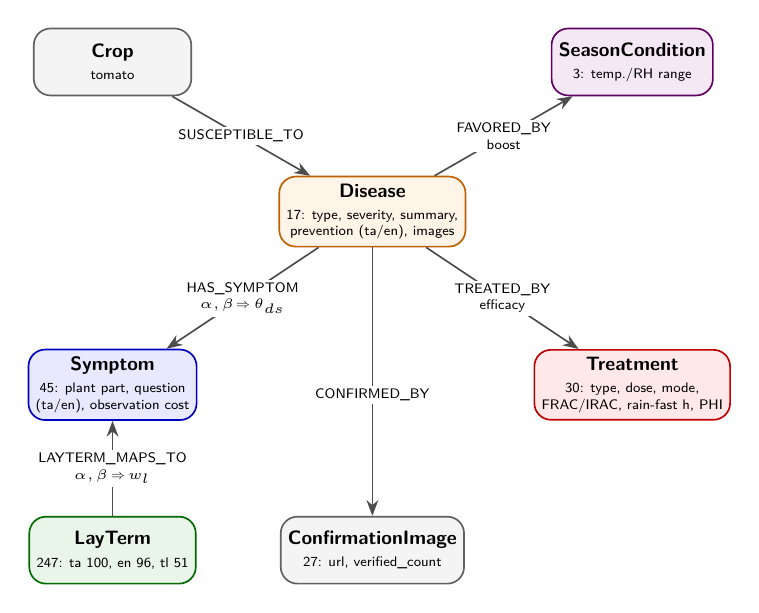
\begin{tikzpicture}[
  font=\sffamily\scriptsize, >=Stealth,
  ent/.style={draw=#1!75!black, fill=#1!9, rounded corners=6pt, align=center, inner sep=2.6pt, line width=0.6pt, minimum width=2.0cm, minimum height=0.85cm},
  rel/.style={->, line width=0.6pt, draw=black!70},
  rl/.style={font=\sffamily\tiny, fill=white, inner sep=1pt, align=center},
]
\node[ent=orange] (d) at (0,0) {\textbf{Disease}\\ {\tiny 17: type, severity, summary,}\\[-2pt] {\tiny prevention (ta/en), images}};
\node[ent=gray] (c) at (-3.3,1.9) {\textbf{Crop}\\ {\tiny tomato}};
\node[ent=violet] (w) at (3.3,1.9) {\textbf{SeasonCondition}\\ {\tiny 3: temp./RH range}};
\node[ent=blue] (s) at (-3.3,-2.2) {\textbf{Symptom}\\ {\tiny 45: plant part, question}\\[-2pt] {\tiny (ta/en), observation cost}};
\node[ent=red] (t) at (3.3,-2.2) {\textbf{Treatment}\\ {\tiny 30: type, dose, mode,}\\[-2pt] {\tiny FRAC/IRAC, rain-fast h, PHI}};
\node[ent=gray] (i) at (0,-4.3) {\textbf{ConfirmationImage}\\ {\tiny 27: url, verified\_count}};
\node[ent=green!55!black] (l) at (-3.3,-4.3) {\textbf{LayTerm}\\ {\tiny 247: ta 100, en 96, tl 51}};

\draw[rel] (c) -- node[rl]{SUSCEPTIBLE\_TO} (d);
\draw[rel] (d) -- node[rl]{FAVORED\_BY\\ {\tiny boost}} (w);
\draw[rel] (d) -- node[rl]{HAS\_SYMPTOM\\ {\tiny $\alpha,\beta \Rightarrow \theta_{ds}$}} (s);
\draw[rel] (d) -- node[rl]{TREATED\_BY\\ {\tiny efficacy}} (t);
\draw[rel] (d) -- node[rl, pos=0.55]{CONFIRMED\_BY} (i);
\draw[rel] (l) -- node[rl]{LAYTERM\_MAPS\_TO\\ {\tiny $\alpha,\beta \Rightarrow w_l$}} (s);
\end{tikzpicture}
}
  \caption{Knowledge-graph schema with node counts. \textsf{HAS\_SYMPTOM} and \textsf{LAYTERM\_MAPS\_TO} weights are Beta posteriors that are updated by confirmed field outcomes.}
  \label{fig:schema}
\end{figure}

\begin{table}[t]
  \caption{Contents of the knowledge graph}
  \label{tab:kg}
  \centering
  \footnotesize
  \begin{tabular}{@{}lr>{\raggedright\arraybackslash}p{4.15cm}@{}}
    \toprule
    Element & Count & Notes \\
    \midrule
    Diseases and pests & 17 & 7 fungal, 5 pest, 2 viral, 2 bacterial, 1 physiological \\
    Symptoms & 45 & 22 leaf, 8 fruit, 6 whole-plant, 4 pest, 3 stem, 1 root, 1 flower \\
    Lay-terms & 247 & 100 Tamil, 96 English, 51 Tanglish \\
    Treatments & 30 & 12 cultural, 10 chemical, 8 organic \\
    \textsf{HAS\_SYMPTOM} & 131 & 7.7 symptoms per disease on average \\
    \textsf{TREATED\_BY} & 65 & efficacy-weighted \\
    Reference photos & 27 & 3 for each of 9 diseases \\
    \textsf{FAVORED\_BY} & 18 & 3 season conditions \\
    \bottomrule
  \end{tabular}
\end{table}

\subsection{Sources and curation}
Symptoms, favourable conditions and treatments for nine diseases are drawn from a tomato disease dataset compiled from more than 40 authoritative sources~\cite{jagtap2025}; the remaining entries are standard extension guidance and are labelled as such in the graph and the user interface. Of the 30 treatments, 21 cite the dataset. Tamil lay-terms were written by the authors, including the 28 phrases of the original prototype, and the graph grows at run time through expert curation (Section~\ref{sec:learning}). A referential-integrity validator checks the graph before every load.

\subsection{Weights as Beta posteriors}
A seeded weight $w_0$ is stored as $\mathrm{Beta}(\alpha,\beta)$ with $\alpha = K w_0$, $\beta = K(1-w_0)$ and prior strength $K=20$ pseudo-observations, so that
\begin{equation}
  \theta_{ds} = \frac{\alpha_{ds}}{\alpha_{ds}+\beta_{ds}} .
  \label{eq:beta}
\end{equation}
Updates add fractional evidence to $\alpha$ or $\beta$, keeping weights in $(0,1)$, reversible and auditable.

\subsection{Treatment application attributes}
Every sprayable treatment carries the attributes required for weather-aware advice (Table~\ref{tab:treat}): mode (contact, systemic, biological, botanical), FRAC/IRAC group~\cite{frac,irac}, dry hours needed before rain, maximum application temperature, preferred time of day, a numeric dose and a repeat interval. Rain-fastness of contact protectants is set conservatively to 4\,h, since reported drying times range from 1.5--2\,h to 6\,h on product labels and mancozeb deposits are partly washed off by moderate rain~\cite{grapepath}; the 32\,$^\circ$C limit for sulfur follows reported phytotoxicity above that temperature~\cite{awri2021}.

\begin{table}[t]
  \caption{Application attributes of selected treatments}
  \label{tab:treat}
  \centering
  \footnotesize
  \setlength{\tabcolsep}{2.5pt}
  \begin{tabular}{@{}>{\raggedright\arraybackslash}p{2.05cm}lllll@{}}
    \toprule
    Treatment & Mode & Group & Dry & $T_{\max}$ & Dose \\
    \midrule
    Mancozeb 75\% WP & contact & M3 & 4\,h & 35\,$^\circ$C & 3\,g/L \\
    Azoxystrobin + difenoconazole & systemic & 11+3 & 2\,h & 35\,$^\circ$C & 200\,mL/ac \\
    Wettable sulfur & contact & M2 & 3\,h & 32\,$^\circ$C & 2\,g/L \\
    \emph{B.~thuringiensis} & biological & 11A$^\dagger$ & 2\,h & 35\,$^\circ$C & 2\,g/L$^\ddagger$ \\
    Neem oil & botanical & -- & 3\,h & 32\,$^\circ$C & 5\,mL/L$^\ddagger$ \\
    \bottomrule
    \multicolumn{6}{@{}p{0.98\columnwidth}@{}}{\scriptsize Group: FRAC code, $^\dagger$IRAC code. Dry: rain-free hours needed after spraying. $^\ddagger$Evening application.}
  \end{tabular}
\end{table}

% =====================================================================
\section{Multilingual Symptom Understanding}
\label{sec:nlu}

\subsection{Concept lexicon}
Tamil, English and Tanglish surface forms map to 95 language-independent concepts through a lexicon of 944 forms (e.g.\ \ta{தூள்}, \ta{பொடி}, \emph{powder}, \emph{podi} $\rightarrow$ \textsc{powder}). Because Tamil is agglutinative (\ta{இலை}, \ta{இலையில்}, \ta{இலைகளில்}), a Tamil token matches the longest lexicon stem it begins with when the remaining suffix has at most eight code points; Latin tokens match exactly or by a stem with at most four trailing characters, with a typo-tolerant fallback (normalised edit similarity $\geq 0.88$) for tokens of five or more characters. Multi-word forms are matched first, which also lets fixed negative idioms such as \ta{காய் பிடிக்கலை} (``fruits are not setting'') be read as symptoms rather than as negations.

\subsection{Negation and clauses}
Text is split into clauses at punctuation and contrastive conjunctions (\ta{ஆனா}, \emph{but}). Tamil negators follow what they negate, so \ta{இல்லை} and negative verb endings such as \mbox{\ta{-க்கலை}} negate the preceding content words; English negators (\emph{no}, \emph{not}, \emph{without}) negate up to three following words. Negated concepts form a separate bag that yields \emph{absent} evidence.

\subsection{IDF-weighted coverage}
Every lay-term phrase $p$ is processed into a concept set $C_p$. Concepts are weighted by inverse document frequency over all phrases~\cite{sparckjones1972}, $w_c = \ln\frac{N+1}{\mathrm{df}_c+1}+1$, so that informative concepts (\textsc{powder}, \textsc{web}) dominate frequent ones (\textsc{leaf}, \textsc{spot}). With $B$ the concepts found in the input and $\sigma(c,B)\in[0,1]$ the best exact or related-concept similarity, the coverage of $p$ is
\begin{equation}
  \mathrm{cov}(p) = \frac{\sum_{c\in C_p} w_c\, \sigma(c,B)}{\sum_{c\in C_p} w_c}.
  \label{eq:cov}
\end{equation}
A phrase matches when $\mathrm{cov}(p)\geq 0.6$ \emph{and} the most informative half of its concepts reaches the same coverage. The second condition prevents generic words from matching a specific phrase (``green leaves on the plant'' must not match ``green caterpillar on the plant''). When the input's negated concepts account for at least a quarter of the phrase weight, the match yields \emph{absent} evidence. The match strength is $s=\mathrm{cov}(p)\,w_l$, and each symptom keeps its strongest match. Fig.~\ref{fig:nlu} traces an example.

\begin{figure}[t]
  \centering
  \resizebox{\columnwidth}{!}{% Worked example of the concept-level NLU (Fig. 3). Values from the implementation.
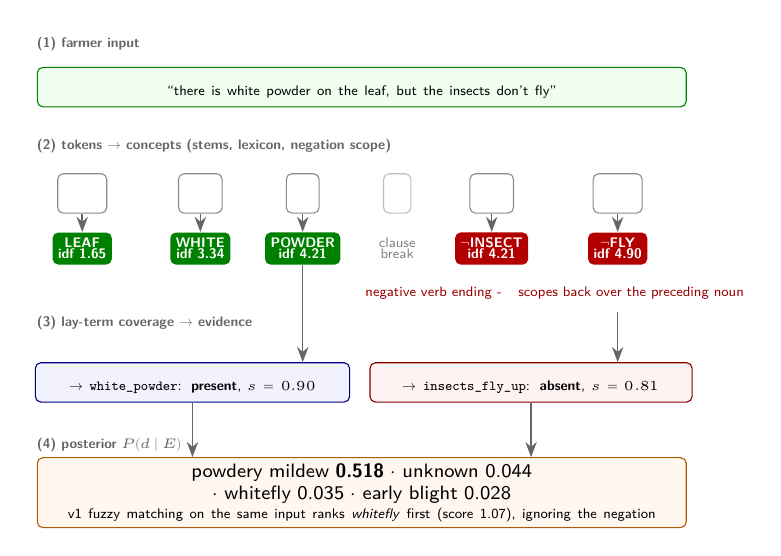
\begin{tikzpicture}[
  font=\sffamily\scriptsize, >=Stealth,
  tok/.style={draw=black!45, rounded corners=2pt, fill=white, inner sep=2pt, minimum height=0.5cm, align=center},
  con/.style={rounded corners=2pt, fill=#1, inner sep=2pt, align=center, font=\sffamily\tiny\bfseries, text=white},
  stp/.style={font=\sffamily\tiny\bfseries, text=black!60, anchor=west},
  arr/.style={->, line width=0.55pt, draw=black!60},
]
% input
\node[stp] at (-4.25, 0.55) {(1) farmer input};
\node[tok, text width=8.1cm, fill=green!6, draw=green!50!black] (in) at (0, 0) {\ta{இலையில் வெள்ளை தூள் இருக்கு ஆனா பூச்சி பறக்கலை}\\[-1pt] {\tiny ``there is white powder on the leaf, but the insects don't fly''}};

% tokens -> concepts
\node[stp] at (-4.25, -0.75) {(2) tokens $\to$ concepts (stems, lexicon, negation scope)};
\node[tok] (t1) at (-3.55,-1.35) {\ta{இலையில்}};
\node[tok] (t2) at (-2.05,-1.35) {\ta{வெள்ளை}};
\node[tok] (t3) at (-0.75,-1.35) {\ta{தூள்}};
\node[tok, draw=black!25, text=black!50] (t4) at (0.45,-1.35) {\ta{ஆனா}};
\node[tok] (t5) at (1.65,-1.35) {\ta{பூச்சி}};
\node[tok] (t6) at (3.25,-1.35) {\ta{பறக்கலை}};
\node[con=green!50!black] (c1) at (-3.55,-2.05) {LEAF\\[-2pt]\tiny idf 1.65};
\node[con=green!50!black] (c2) at (-2.05,-2.05) {WHITE\\[-2pt]\tiny idf 3.34};
\node[con=green!50!black] (c3) at (-0.75,-2.05) {POWDER\\[-2pt]\tiny idf 4.21};
\node[font=\sffamily\tiny, text=black!50, align=center] at (0.45,-2.05) {clause\\[-2pt]break};
\node[con=red!70!black] (c5) at (1.65,-2.05) {$\neg$INSECT\\[-2pt]\tiny idf 4.21};
\node[con=red!70!black] (c6) at (3.25,-2.05) {$\neg$FLY\\[-2pt]\tiny idf 4.90};
\foreach \i in {1,2,3,5,6} \draw[arr] (t\i) -- (c\i);
\node[font=\sffamily\tiny, text=red!60!black, align=center] at (2.45,-2.62) {negative verb ending \ta{-கலை} scopes back over the preceding noun};

% lay-term matches
\node[stp] at (-4.25, -3.0) {(3) lay-term coverage $\to$ evidence};
\node[tok, text width=3.85cm, fill=blue!5, draw=blue!50!black] (m1) at (-2.15,-3.75) {\ta{இலையில் வெள்ளை பொடி}\\[-1pt]{\tiny $\to$ \texttt{white\_powder}: \textbf{present}, $s=0.90$}};
\node[tok, text width=3.95cm, fill=red!5, draw=red!50!black] (m2) at (2.15,-3.75) {{\small\ta{வெள்ளை சிறு பூச்சிகள் பறக்கும்}}\\[-1pt]{\tiny $\to$ \texttt{insects\_fly\_up}: \textbf{absent}, $s=0.81$}};
\draw[arr] (c3.south) -- (m1.north -| c3.south);
\draw[arr] (c6.south) ++(0,-0.6) -- (m2.north -| c6.south);

% posterior
\node[stp] at (-4.25, -4.55) {(4) posterior $P(d\mid E)$};
\node[tok, text width=8.1cm, fill=orange!6, draw=orange!70!black] (p) at (0,-5.15) {powdery mildew \textbf{0.518} $\cdot$ unknown 0.044 $\cdot$ whitefly 0.035 $\cdot$ early blight 0.028\\[-1pt]
{\tiny v1 fuzzy matching on the same input ranks \emph{whitefly} first (score 1.07), ignoring the negation}};
\draw[arr] (m1.south) -- (p.north -| m1.south);
\draw[arr] (m2.south) -- (p.north -| m2.south);
\end{tikzpicture}
}
  \caption{Worked example. The Tamil input contains a synonym of the lay-term (\ta{தூள்} vs.\ \ta{பொடி}, both \textsc{powder}) and a negated clause. The concept matcher produces one present and one absent symptom, and the posterior favours powdery mildew. All values are produced by the implementation.}
  \label{fig:nlu}
\end{figure}

\subsection{Speech and LLM entity linking}
For voice input, the recording is converted to 16\,kHz mono WAV in the browser and sent to a multimodal LLM (Gemini~\cite{gemini2023}) with a JSON schema whose symptom and treatment fields are \emph{enumerations of KG identifiers}. The model returns a verbatim transcript, linked symptoms with a confidence and the quoted words, severity, the estimated share of affected plants, duration, crop stage and products already sprayed; it is explicitly instructed not to diagnose. The output is validated (unknown identifiers dropped, numbers clamped), the transcript is also passed through the concept matcher, and LLM-linked symptoms are used only where the matcher found nothing. The LLM thus widens recall without being able to introduce a disease or a dosage that is not in the curated graph. Without an API key the system falls back to browser speech recognition, and severity and extent are still extracted from plain words (e.g.\ \ta{கொஞ்சம்}, ``a little'' $\rightarrow$ mild). This component is implemented and unit-tested with recorded responses but was \emph{not} part of the quantitative evaluation.

% =====================================================================
\section{Bayesian Diagnosis and Information-Gain Dialogue}
\label{sec:inference}

\subsection{Hypotheses and evidence}
The hypothesis space $\mathcal{H}$ contains the 17 diseases and an explicit \unk{} hypothesis (``a problem not in the graph'') with $\theta_{\unk,s}=0.12$ for every symptom. Each piece of evidence $e$ is a report that symptom $s_e$ is present or absent, with a reliability $c_e$: for text $c=\mathrm{clip}(0.5+0.45\,s,\,0.55,\,0.95)$; for answers $c=0.92$ (yes) or $0.90$ (no); for tapped symptoms $c=0.90$; for LLM links $c=\mathrm{clip}(0.5+0.4\,\kappa,\,0.55,\,0.90)$ with model confidence $\kappa$. A direct answer overrides inferred evidence for the same symptom. With $\theta=\theta_{hs}$, or a leak value of 0.02 when the KG has no edge, the report likelihood is
\begin{align}
  P(e^{+}\mid h) &= c\,\theta + \lambda\,(1-c)(1-\theta), \label{eq:pos}\\
  P(e^{-}\mid h) &= c\,(1-\theta) + (1-c)\,\theta, \label{eq:neg}
\end{align}
where $\lambda=0.3$ makes false alarms rarer than misses: farmers overlook symptoms more often than they invent a specific one. A weak language match therefore moves the posterior only slightly, which bounds the damage of matching errors.

\subsection{Priors and photo fusion}
The prior is $P(h)\propto f_h$ with $f_\unk=0.6$ and, for a disease, either a calendar-season boost $f_d = 1 + b_d$ from \textsf{FAVORED\_BY} edges or, when the location is known, the weather-driven factor of Section~\ref{sec:advisory}. A leaf photo enters as a tempered likelihood
\begin{equation}
  L_{\mathrm{img}}(d) = \begin{cases} \max(p_d,\,0.02)^{\tau} & d \text{ in the classifier's classes},\\ 0.05^{\tau} & \text{otherwise,} \end{cases}
  \label{eq:photo}
\end{equation}
where $p_d$ is the calibrated class probability and $\tau=0.6$, reduced to 0.25 when a quality check fails or $\max_d p_d<0.5$, and to 0 when no leaf is detected. The posterior is
\begin{equation}
  P(h\mid E) \propto P(h)\, L_{\mathrm{img}}(h) \prod_{e\in E} P(e\mid h).
  \label{eq:post}
\end{equation}

\subsection{Cost-aware expected information gain}
For an unobserved symptom $s$, let $\pi=P(\cdot\mid E)$ and $\pi^{a}$ the posterior after answer $a\in\{\text{yes},\text{no}\}$ with reliability 0.92. The expected information gain is
\begin{equation}
  \EIG(s) = H(\pi) - \sum_{a} P(a\mid E)\, H(\pi^{a}),
  \label{eq:eig}
\end{equation}
with $H$ the Shannon entropy in bits~\cite{lindley1956}, and the next question maximises $\EIG(s)\,(1-\mathrm{cost}_s)$. Dialogue stops when the best disease reaches 0.85, after six questions, or when no question offers more than 0.03\,bits (Algorithm~\ref{alg:dialogue}). The farmer may also answer ``not sure'' or ask for the result at any time.

\begin{algorithm}[t]
\caption{Interactive diagnosis}
\label{alg:dialogue}
\footnotesize
\begin{algorithmic}[1]
\Require text $x$, optional photo, location, tapped symptoms
\Ensure diagnosis with explanation, or an abstention
\State $E \gets$ \textsc{Match}$(x)$ $\cup$ tapped symptoms $\cup$ LLM links \Comment{Sec.~\ref{sec:nlu}}
\State $P(h) \gets$ \textsc{Prior}(location, weather, outbreaks) \Comment{Sec.~\ref{sec:advisory}}
\If{$E=\emptyset$ \textbf{and} no photo} \State \Return ask the farmer to tap symptoms; log $x$ for experts \EndIf
\For{$k = 1,\dots,6$}
  \State compute $\pi = P(h\mid E)$ by \eqref{eq:post}
  \If{$\max_{d}\pi_d \geq 0.85$} \textbf{break} \EndIf
  \State $s^\star \gets \arg\max_{s\notin E} \EIG(s)\,(1-\mathrm{cost}_s)$
  \If{$\EIG(s^\star) < 0.03$} \textbf{break} \EndIf
  \State ask the question of $s^\star$; add the answer to $E$ unless ``not sure''
\EndFor
\State $d_1, d_2 \gets$ two most probable diseases
\If{$\pi_\unk > \pi_{d_1}$ \textbf{or} $\pi_{d_1} < 0.35$} \State \Return abstain: compare reference photos, contact an expert \EndIf
\State \Return $d_1$, $\pi_{d_1}$, evidence ranked by $|\log P(e\mid d_1) - \log P(e\mid d_2)|$, advisory
\end{algorithmic}
\end{algorithm}

\subsection{Explanations}
For the top disease $d_1$ and the runner-up $d_2$, each evidence item is shown with its log-likelihood ratio $\log P(e\mid d_1)-\log P(e\mid d_2)$, labelled as supporting or contradicting, together with the farmer's own words, the lay-term it matched and the KG weight $\theta_{d_1 s}$. The strongest unobserved symptoms of $d_1$ are listed as things to check next.

% =====================================================================
\section{Weather- and Location-Aware Advisory}
\label{sec:advisory}

\subsection{Disease-risk models}
Given a location (GPS or a district, always rounded to a 0.05$^\circ$ grid of about 5\,km), the system retrieves seven days of hourly history and three days of forecast~\cite{openmeteo}. Relative humidity $\geq$90\% serves as the leaf-wetness proxy, as in operational TOM-CAST implementations~\cite{frost2015}.
\emph{Late blight} uses the Hutton criteria~\cite{ahdb_hutton}: a day qualifies when the minimum temperature is $\geq$10\,$^\circ$C and at least six hours have RH$\geq$90\%; with $P$ the number of consecutive qualifying day pairs in the last week, $H$ the qualifying days and $F$ an indicator of a forecast pair,
\begin{equation}
  r_{\mathrm{LB}} = \min\bigl(1,\,0.45P + 0.15H + 0.3F\bigr)\, g(\bar T),
\end{equation}
where $g$ is 1 for a mean temperature of 12--23\,$^\circ$C (the dataset gives 18--23\,$^\circ$C as the fastest-spread range~\cite{jagtap2025}) and decreases linearly to 0.1 at 30\,$^\circ$C, because the criteria were calibrated in a temperate climate. \emph{Early blight} sums TOM-CAST daily severity values~\cite{madden1978,frost2015} over the last seven days and uses $r_{\mathrm{EB}}=\min(1,\mathrm{DSV}_7/15)$. Eleven further diseases use transparent rules that count hours meeting favourable temperature and humidity conditions (e.g.\ $T\geq30$\,$^\circ$C and RH$<$50\% for spider mites), taken from~\cite{jagtap2025} where the dataset covers the disease (septoria, leaf mold, target spot, spider mite, leaf miner, leaf curl virus) and from general guidance otherwise; they are capped at 0.8 so that heuristics never claim the certainty of the published models. Four diseases without a weather signal (fruit borer, root-knot nematode, Fusarium wilt, mosaic virus) receive no model. Risks are shown as a weekly early warning, and replace the calendar season in the prior as $f_d = 1 + 1.5\,r_d$, with unmodelled diseases receiving the mean factor.

\subsection{Community outbreak signal}
Confirmed diagnoses with a location become reports. For a farmer, the count $n_d$ of reports of disease $d$ within 30\,km in the last 21 days multiplies the prior by $1+0.2\min(n_d,5)$ and triggers an alert; an expert map shows all reports.

\subsection{Spray windows}
An hour is suitable for a product when it falls in the product's application hours (daylight, or 16:00--19:00 for UV-sensitive biologicals and oils), it is not raining, no hour within the product's rain-fast period has $\geq$0.3\,mm of rain or $\geq$60\% rain probability, the wind is below 20\,km/h~\cite{agvic_wind}, the temperature is below the product limit, and RH is below 97\%. The earliest run of at least two suitable hours in the next 72\,h is reported, with a caution for wind of 15--20\,km/h. Every treatment is labelled \emph{OK now}, \emph{wait} (with the reason and the next window) or \emph{not in the next three days}.

\subsection{Severity-adaptive, resistance-aware plan}
Treatments are ranked by efficacy adjusted for severity (mild: cultural $+0.3$, organic $+0.2$, chemical $-0.3$; severe: chemical $+0.25$, cultural $+0.1$, organic $-0.1$), for rain expected within 24\,h (systemic $+0.1$, contact $-0.05$) and for resistance (a product sharing a FRAC/IRAC group with a recently sprayed one: $-0.4$). Previously sprayed products named by the farmer are fuzzy-matched to KG treatments; the plan states when to switch groups and when a product does not target the diagnosed problem, and that viral diseases have no cure. The share of affected plants sets the scope (below 10\%: treat or remove those plants; below 40\%: the patch; otherwise the field). A dated schedule alternates resistance groups at the products' repeat intervals and is exported as an iCalendar file; a calculator converts doses to a 16\,L knapsack tank and to the farmer's area in cents or acres.

% =====================================================================
\section{Learning from Farmer Feedback}
\label{sec:learning}

After a diagnosis the farmer confirms it, picks the correct disease from reference photos, rejects it, or is unsure. Only confirmed or corrected outcomes update weights: a bare rejection tells us that the answer was wrong, not which answer is right, and decaying the predicted disease's edges on rejection, as the prototype did, penalises edges that may be correct. For the true disease $d^\star$ and each evidence item with reliability $c$, let $\omega = 2(c-0.5)$. If $(d^\star,s)$ exists, a present report adds $\omega$ to $\alpha$ and an absent report adds $\omega$ to $\beta$. A present symptom with $\omega\geq0.6$ and no edge creates a \emph{suggested edge} for expert review. For a text match through lay-term $l$, $\alpha_l$ grows by $\omega/2$ if $s$ is a symptom of $d^\star$ and $\beta_l$ otherwise. Descriptions that matched nothing are queued in an expert console, where mapping one to a symptom creates a new LayTerm node immediately; Fig.~\ref{fig:expert} shows the console.

\begin{figure}[t]
  \centering
  \subfloat[Knowledge-graph explorer focused on late blight; the tooltip gives the Tamil name (diseases red, symptoms green, treatments gold, edge width = weight)]{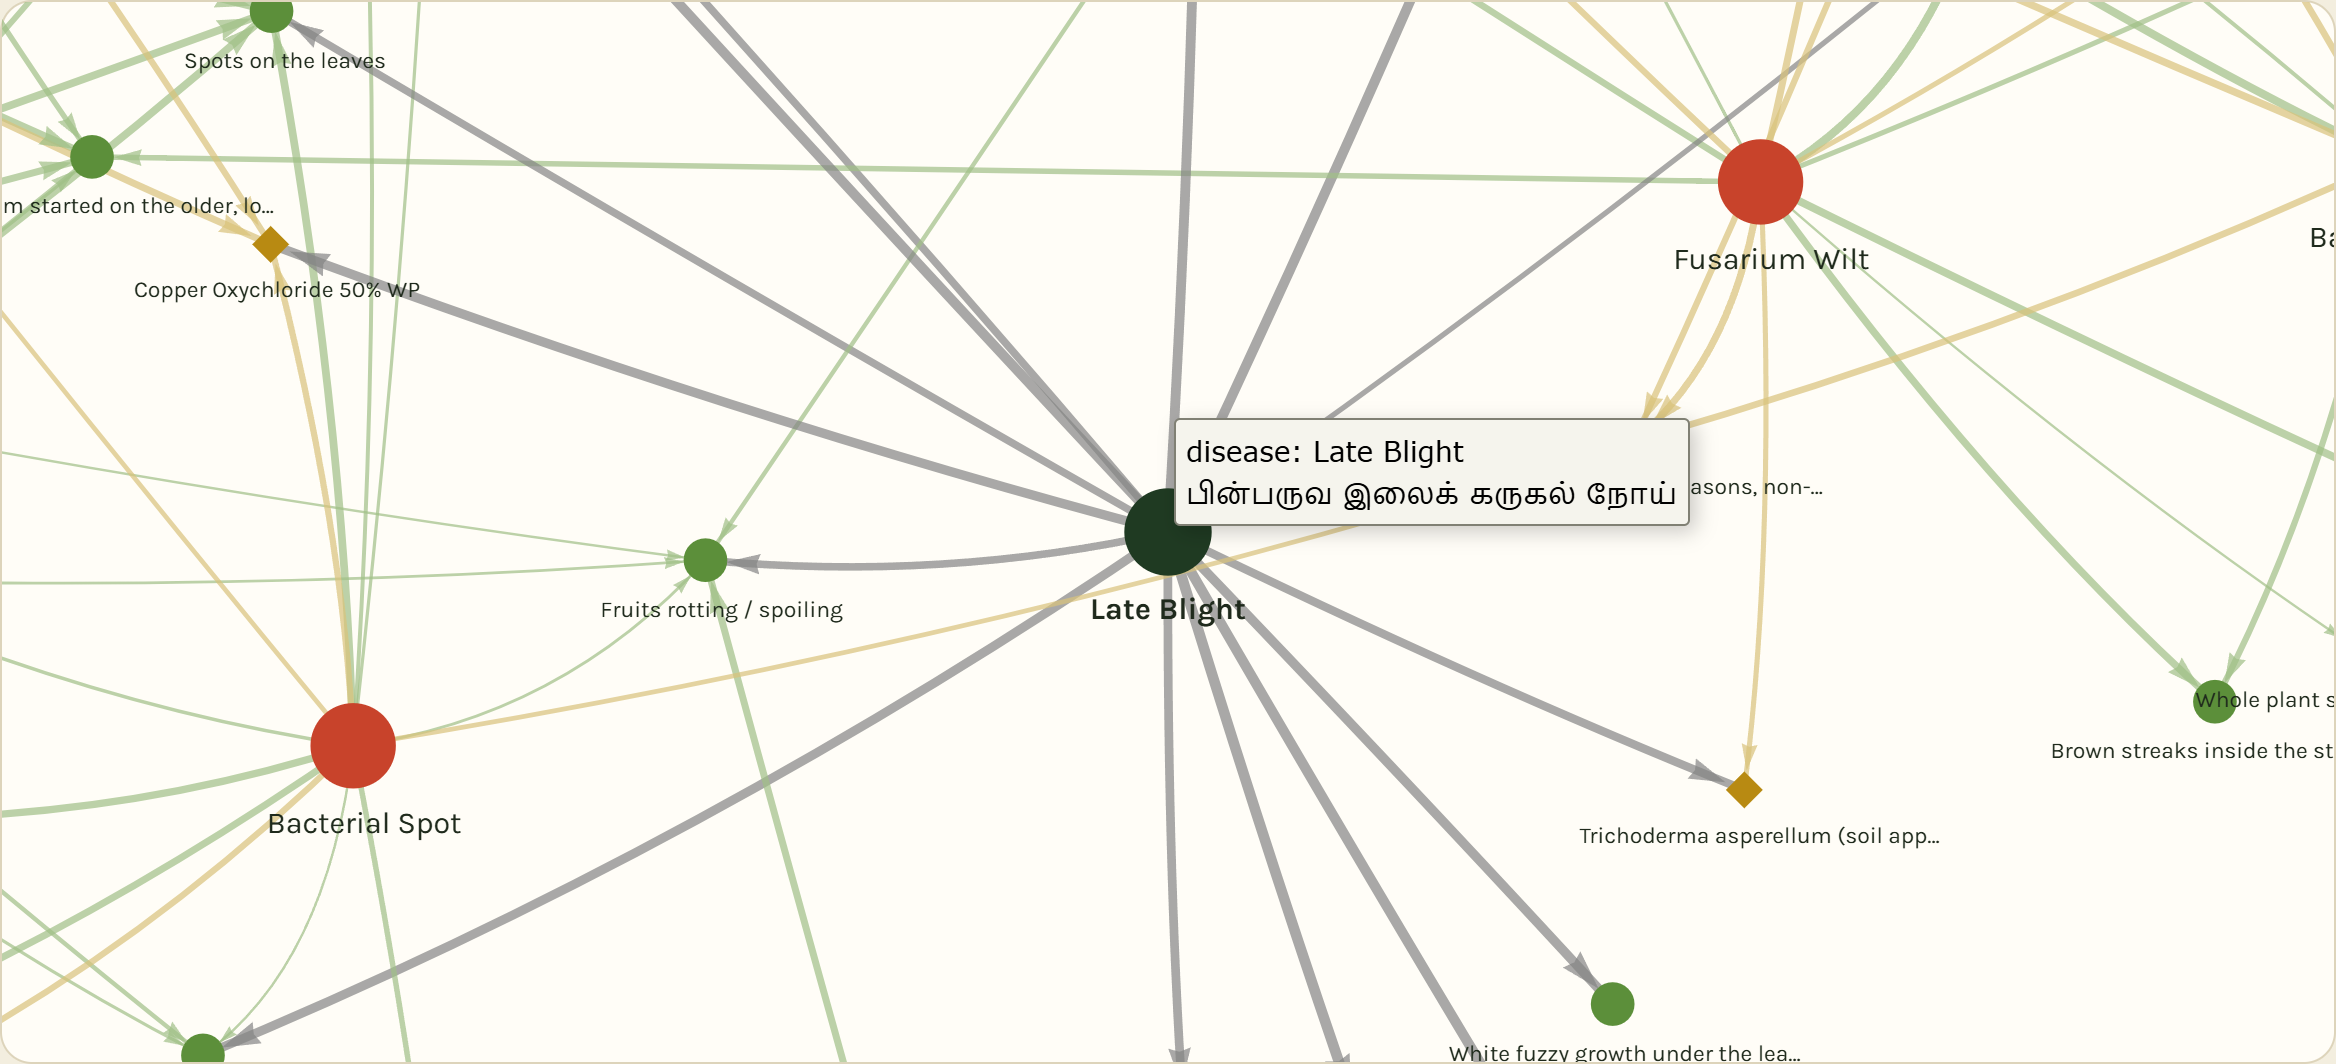
\includegraphics[width=\columnwidth]{figures/screens/g_graph.png}}\\
  \subfloat[Community outbreak map (simulated demonstration reports)]{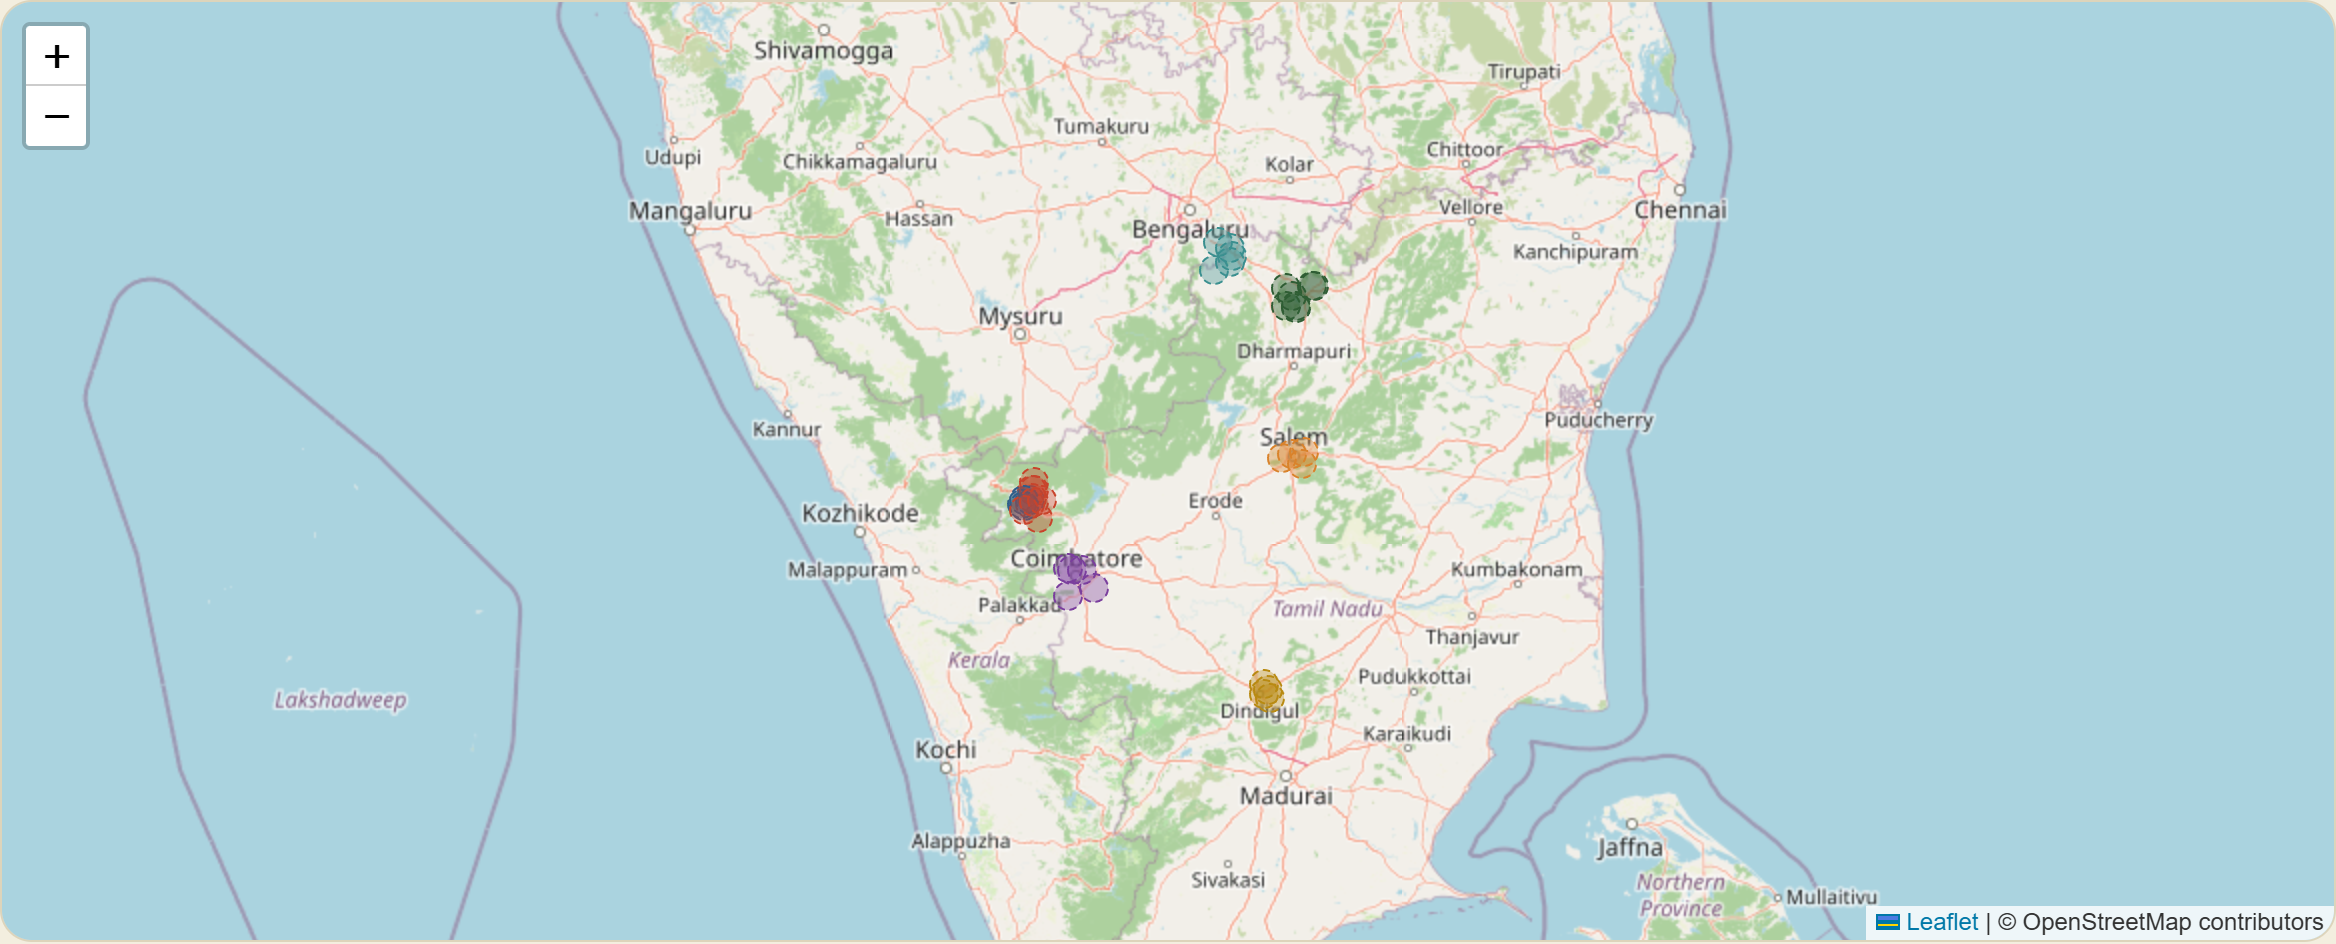
\includegraphics[width=\columnwidth]{figures/screens/g_map.png}}
  \caption{Expert console. Edge thickness encodes the KG weight; the console also lists unmatched farmer phrases for curation and the drift of every learned edge weight.}
  \label{fig:expert}
\end{figure}

% =====================================================================
\section{Implementation}
\label{sec:impl}

The back end is a Python/Flask service. The KG is stored in Neo4j~\cite{neo4j} (tested with Neo4j 5.26; AuraDB is supported) or in an embedded store that combines the curated JSON seed with learned state in SQLite; both produce the same in-memory graph, and the service falls back to the embedded store when Neo4j is unreachable. Learned $\alpha,\beta$ are written back onto the Neo4j relationships. The front end is a framework-free progressive web application with Tamil and English interfaces, read-aloud, tap-to-pick symptoms, a disease library, history, sharing and a service worker for weak connectivity (Fig.~\ref{fig:screens}).

The leaf classifier uses a frozen ImageNet MobileNetV3-Large backbone~\cite{howard2019} on a 10-class PlantVillage tomato subset~\cite{hughes2015} (9 diseases and healthy; 1,000 training and 100 validation images per class). Pooled 960-d features of the training images and their mirror images (20,000 vectors) train a 960--256--10 MLP head with dropout 0.3, AdamW~\cite{loshchilov2019} (learning rate $2\times10^{-3}$, weight decay $10^{-3}$, cosine schedule, 40 epochs), label smoothing 0.05~\cite{szegedy2016} and Gaussian feature noise. A softmax temperature ($T=0.523$) is fitted on the validation set~\cite{guo2017}, and the network is exported to ONNX (12.9\,MB) for CPU inference. Validation accuracy is 97.6\% (Fig.~\ref{fig:vision}a); because the epoch and the temperature were selected on the same 1,000 images, this figure is optimistic. Lightweight checks flag dark, over-exposed, blurred and leafless photographs.

The implementation comprises about 3,000 lines of Python, a test suite of 71 tests (including Neo4j integration tests), and reproducible scripts for training, evaluation, figures and screenshots.

\begin{figure*}[t]
  \centering
  \subfloat[Field conditions]{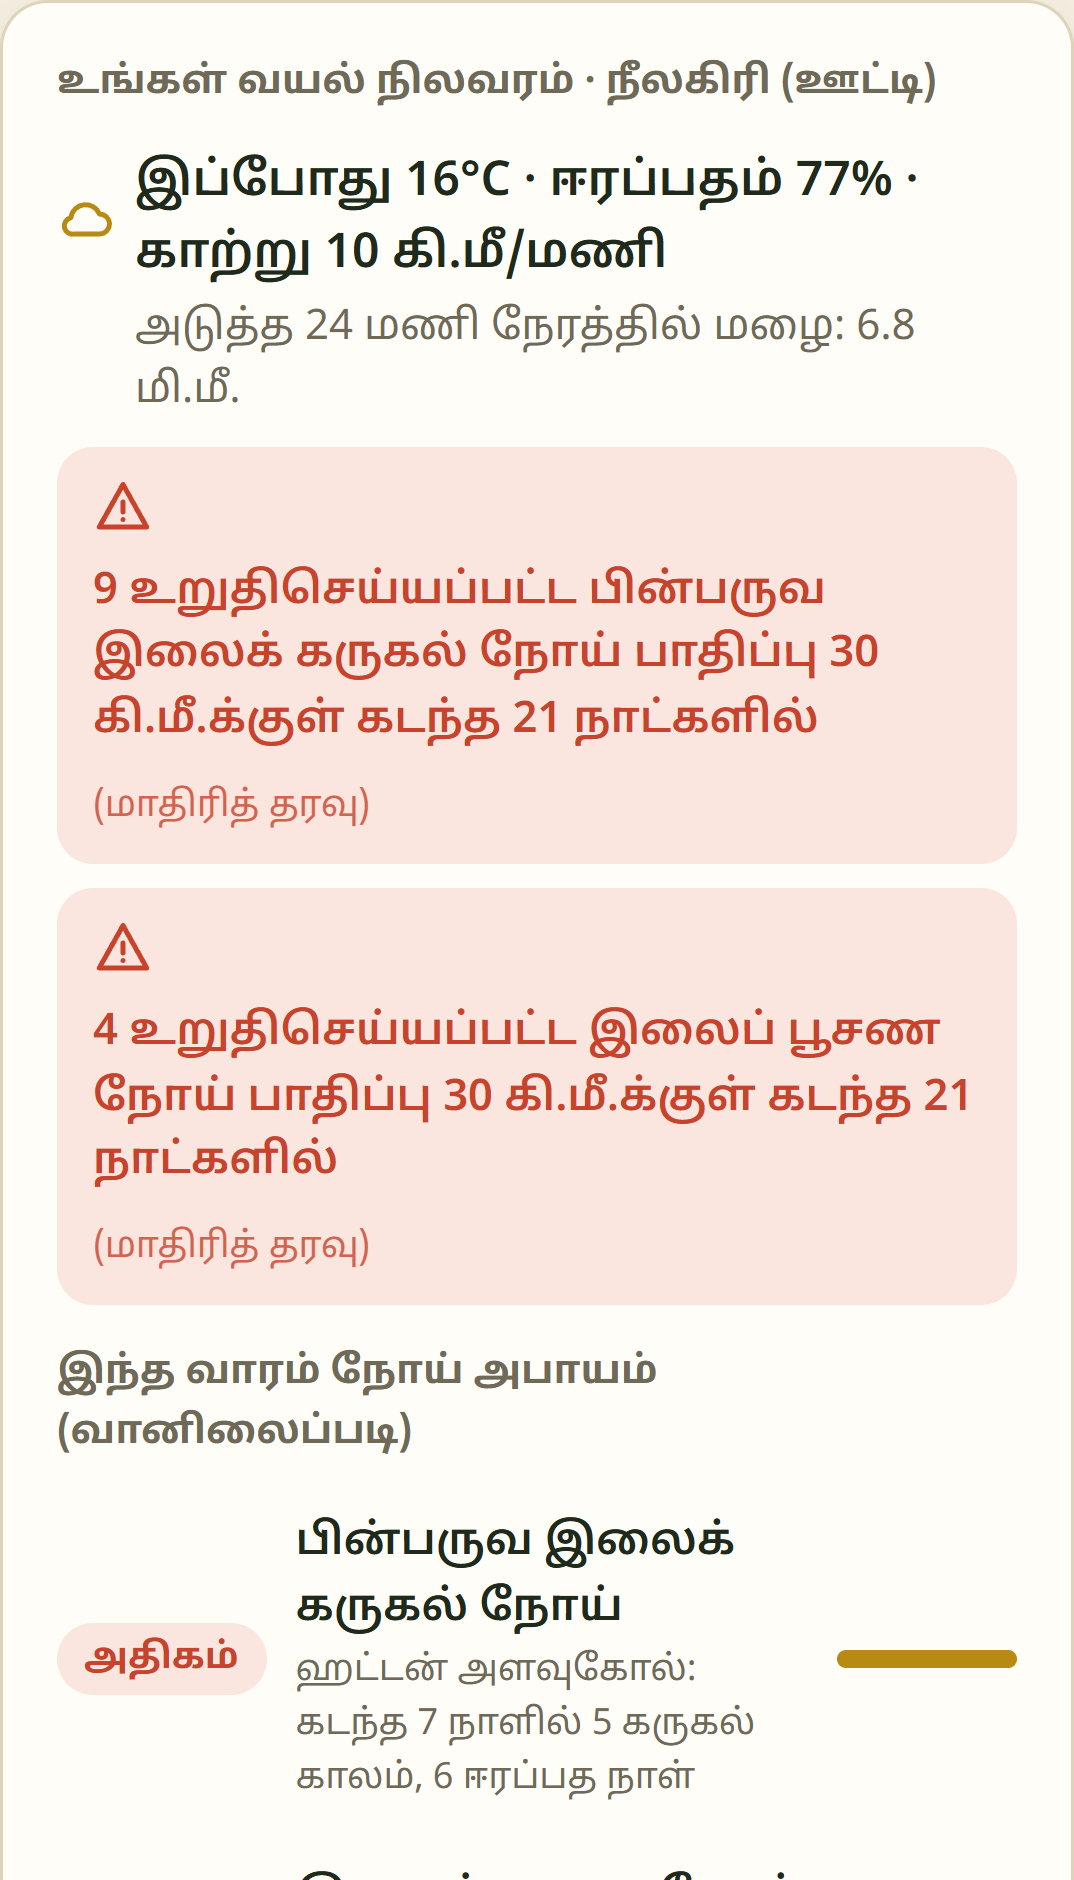
\includegraphics[height=6.1cm]{figures/screens/a_field_top.png}}\hfil
  \subfloat[Information-gain question]{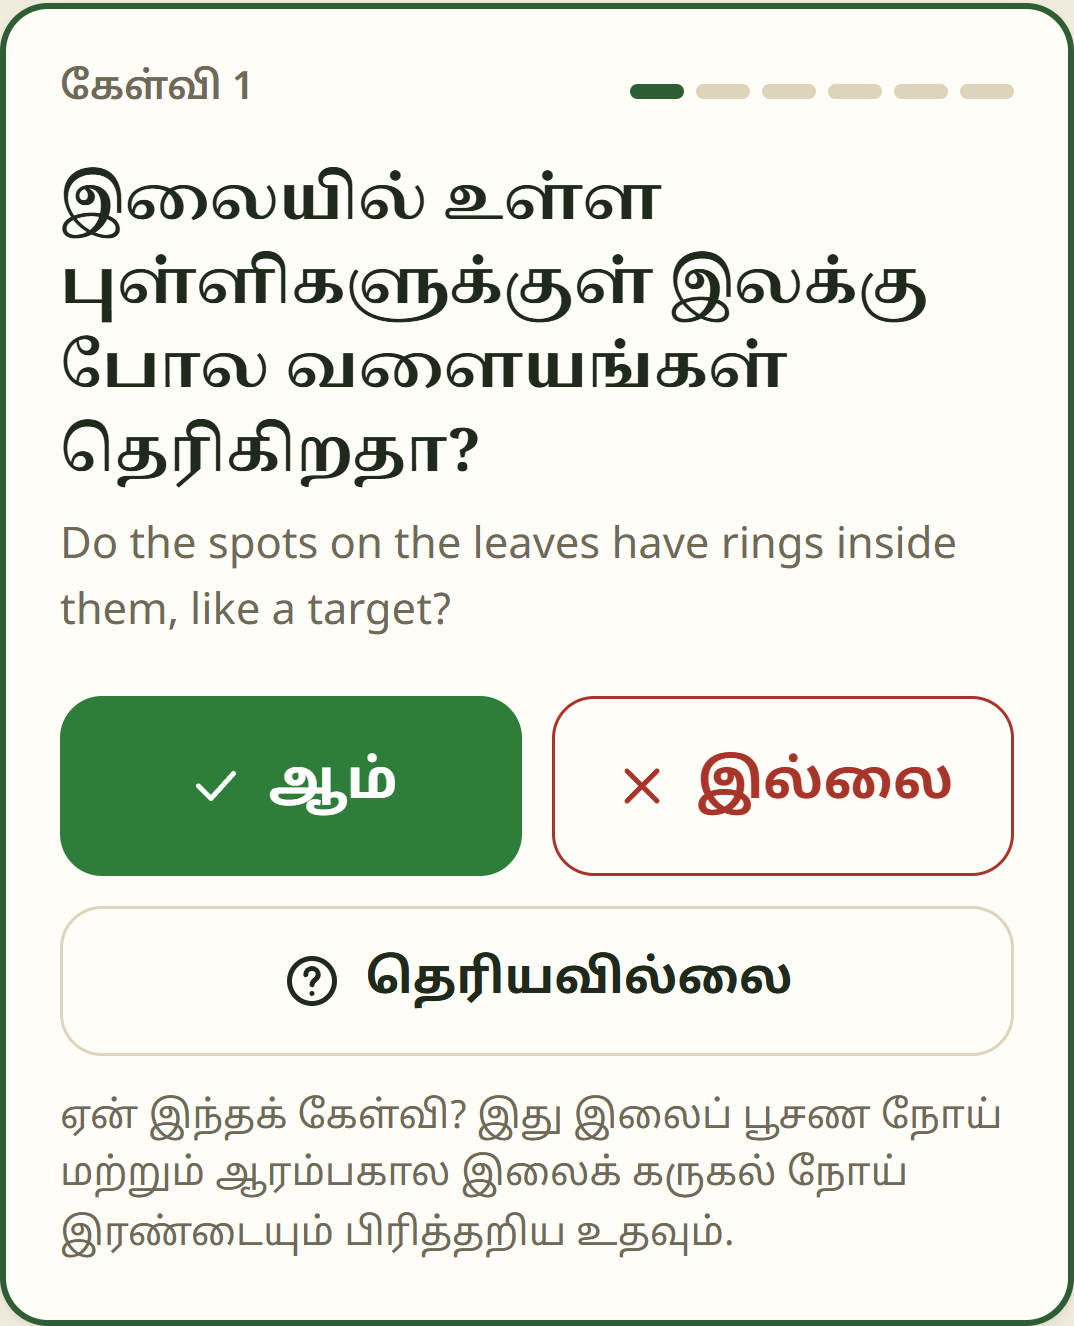
\includegraphics[height=6.1cm]{figures/screens/b_question.png}}\hfil
  \subfloat[Diagnosis]{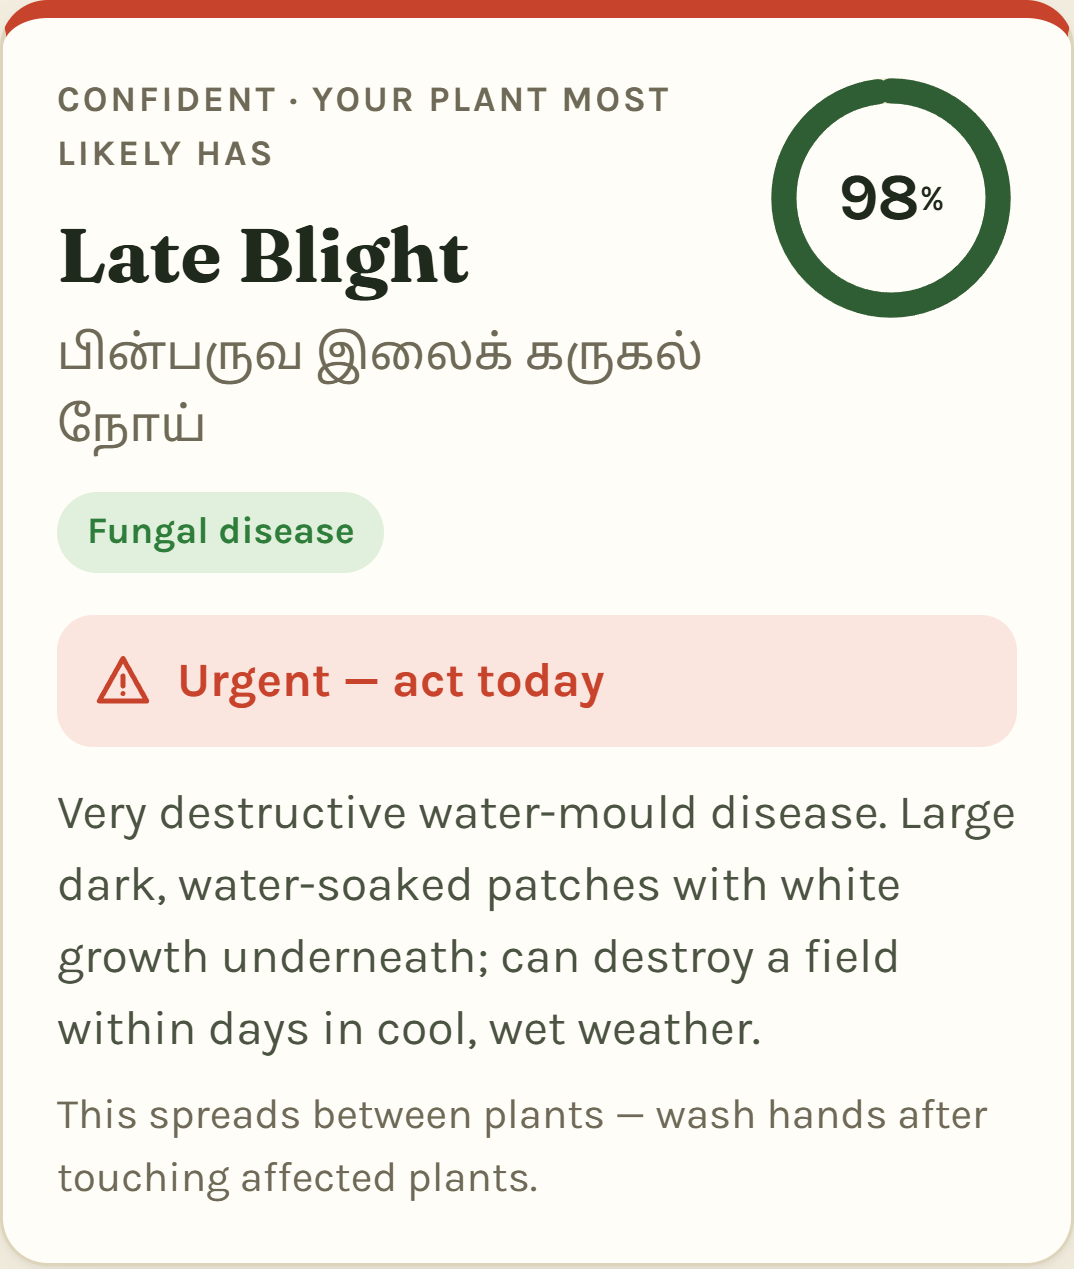
\includegraphics[height=6.1cm]{figures/screens/c_hero.png}}\hfil
  \subfloat[Weather-aware plan]{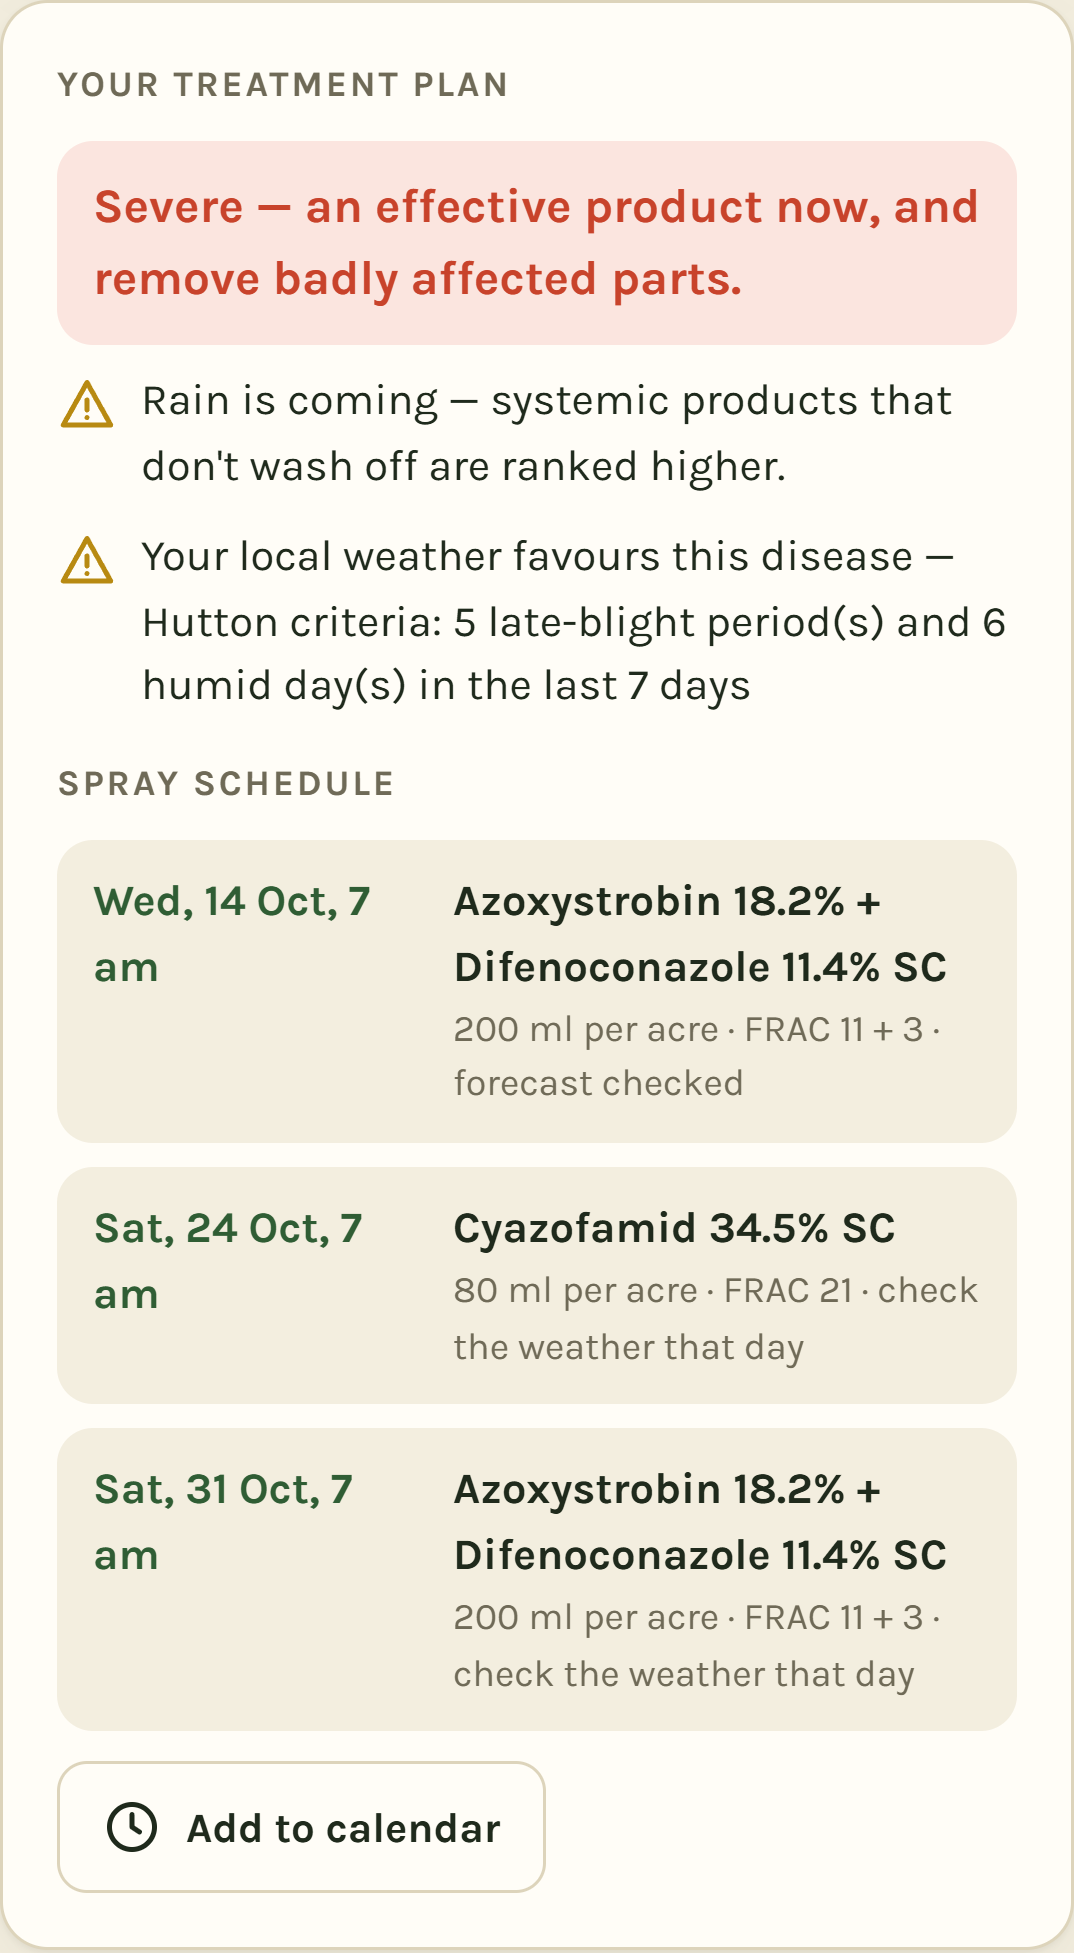
\includegraphics[height=6.1cm]{figures/screens/d_plan.png}}
  \caption{The farmer application on a phone (location: the Nilgiris). (a) Live weather, a weekly risk list led by late blight (Hutton criteria) and outbreak alerts, which are marked as simulated in this demonstration. (b) A question that separates leaf mold from early blight, asked in Tamil with an English subtitle. (c) A confident late-blight diagnosis. (d) Severity-adaptive plan citing the local weather evidence, and a schedule that alternates FRAC groups.}
  \label{fig:screens}
\end{figure*}

% =====================================================================
\section{Evaluation}
\label{sec:eval}

\subsection{Setup}
\emph{Test set.} 85 farmer descriptions, five per disease (two Tamil, two English, one Tanglish: 34/34/17), were written independently of the KG lay-terms, using different wording, partial descriptions and multiple symptoms. \emph{Simulated farmer.} Questions are answered ``yes'' with probability $\theta_{d^\star s}$ for the true disease $d^\star$, or 0.02 when no edge exists, so answers are noisy; each case is run 20 times. We report top-1 and top-3 accuracy, the rate of \emph{confidently wrong} answers (a wrong disease with posterior $\geq0.85$; for the prototype, a non-ambiguous wrong answer), the mean number of questions, and 95\% bootstrap confidence intervals over cases (2,000 resamples)~\cite{efron1993}. \emph{Baselines and ablations} (Table~\ref{tab:main}) all use the same KG: the prototype (whole-phrase fuzzy matching with a 0.55 threshold and additive scoring; its follow-up answers did not affect the ranking, so its final answer equals its text-only answer); the prototype's matcher with our engine; our matcher without questions; random questions; the prototype's question rule (prefer a symptom absent for one of the top-3 candidates, else the largest weight variance) with answers fed back; and the full system with symmetric noise ($\lambda=1$) or without the \unk{} hypothesis.

\begin{table}[t]
  \caption{Diagnostic accuracy on 85 held-out descriptions (20 simulated dialogues each)}
  \label{tab:main}
  \centering
  \footnotesize
  \setlength{\tabcolsep}{2.6pt}
  \begin{tabular}{@{}lcccc@{}}
    \toprule
    Method & Top-1 [95\% CI] & Top-3 & Wrong$^{*}$ & Qs. \\
    \midrule
    v1 prototype & 63.5 [52.9, 74.1] & 85.9 & 10.6 & -- \\
    v1 matching + our engine & 86.4 [82.0, 90.4] & 95.8 & 1.9 & 4.19 \\
    Our matching, no questions & 92.9 [87.1, 97.6] & 100.0 & 0.0 & 0 \\
    \quad + random questions & 95.1 [92.5, 97.3] & 99.9 & 0.5 & 3.58 \\
    \quad + v1 variance rule & 96.3 [93.9, 98.2] & 99.9 & 0.9 & 3.36 \\
    \quad + EIG (\textbf{proposed}) & \textbf{96.8} [94.5, 98.5] & 99.7 & 1.2 & \textbf{2.12} \\
    \midrule
    Proposed, symmetric noise & 96.5 [94.5, 98.2] & 99.7 & 0.1 & 3.79 \\
    Proposed, no \unk{} & 96.6 [94.3, 98.5] & 99.9 & 1.2 & 2.01 \\
    \bottomrule
    \multicolumn{5}{@{}p{0.98\columnwidth}@{}}{\scriptsize All values in \% except Qs.\ (mean number of questions). $^{*}$Confidently wrong: wrong disease reported with posterior $\geq0.85$.}
  \end{tabular}
\end{table}

\subsection{Diagnostic accuracy and ablations}
Table~\ref{tab:main} shows that the language layer is the largest single improvement: replacing whole-phrase fuzzy matching with concept-level matching raises description-only accuracy from 63.5\% to 92.9\%, and the prototype's matcher remains the bottleneck even when paired with our engine (86.4\%). The prototype understood 91.8\% of inputs and was confidently wrong on 10.6\%; the motivating ``white dust'' sentence illustrates why: shared filler words gave weight to unrelated ring-spot lay-terms, and a negated clause was ignored entirely (Fig.~\ref{fig:nlu}). Dialogue adds 3.9 points, and every configuration built on our matcher is confidently wrong on at most 1.2\% of runs. Accuracy is balanced across languages: 96.3\% for Tamil, 96.9\% for English and 97.4\% for Tanglish inputs (prototype: 67.6\%, 52.9\% and 76.5\%). Per disease (Fig.~\ref{fig:perdisease}), the remaining errors concentrate on bacterial spot (75\%) and target spot (89\%); the most frequent confusions are bacterial spot $\to$ target spot and target spot $\to$ early blight, three diseases that genuinely share small dark, ring-forming lesions with yellow halos in the dataset~\cite{jagtap2025}.

\begin{figure}[t]
  \centering
  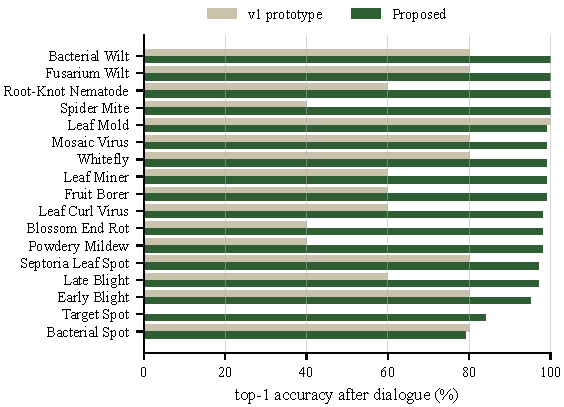
\includegraphics[width=\columnwidth]{figures/per_disease.pdf}
  \caption{Top-1 accuracy per disease after dialogue (five descriptions per disease; 20 dialogues each for the proposed system).}
  \label{fig:perdisease}
\end{figure}

\subsection{Question efficiency}
The accuracy differences between EIG, the variance rule and random questions lie within each other's confidence intervals, so we do not claim that EIG is more accurate. Its benefit is efficiency: it reaches 96.8\% with 2.12 questions, 37\% fewer than the variance rule (3.36) and 41\% fewer than random selection (3.58). Fig.~\ref{fig:budget} fixes the question budget: with three questions, EIG reaches 96.1\% versus 95.9\% for the variance rule and 93.9\% for random questions. Modelling false alarms as rarer than misses ($\lambda=0.3$) saves 44\% of questions relative to symmetric noise (2.12 vs.\ 3.79) at the same accuracy, at the cost of more confidently wrong answers (1.2\% vs.\ 0.1\%), a trade-off that can be tuned with $\lambda$ and the stopping threshold. Fig.~\ref{fig:trace} shows the motivating case: after ``white dust on the leaf'', the first question asks whether insects are present; for whitefly two ``yes'' answers reach 0.93, whereas for powdery mildew the posterior rises steadily as alternatives are excluded and reaches 0.77 (``likely'') after six questions, because powdery mildew has few distinctive symptoms in the KG.

\begin{figure}[t]
  \centering
  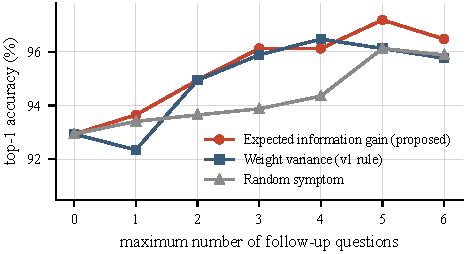
\includegraphics[width=\columnwidth]{figures/budget_curves.pdf}
  \caption{Top-1 accuracy as a function of the maximum number of questions (85 cases $\times$ 10 dialogues per point).}
  \label{fig:budget}
\end{figure}

\begin{figure}[t]
  \centering
  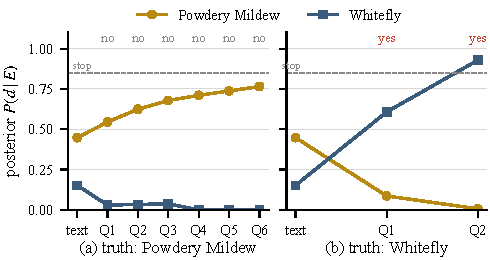
\includegraphics[width=\columnwidth]{figures/dialogue_trace.pdf}
  \caption{Posterior during the dialogue for ``\ta{இலையில் வெள்ளை தூள் போல இருக்கு}'' when the truth is (a) powdery mildew and (b) whitefly; answers are given above the axes. The dashed line is the stopping threshold.}
  \label{fig:trace}
\end{figure}

\subsection{Out-of-scope problems}
Twelve descriptions of problems absent from the KG (frost, hail, herbicide drift, nutrient deficiency, fruit cracking, sun-scald, damping-off, animal damage) were run 20 times each, with the simulated farmer answering ``yes'' with probability 0.15. The system abstained in 82.1\% of runs and was confidently wrong in 6.3\%; 66.7\% of runs abstained because no symptom matched; in deployment such descriptions are queued for expert curation. Removing the \unk{} hypothesis changed these rates only slightly (80.8\% and 6.7\%), so in this setting abstention is driven mainly by the matching threshold and the low-confidence rule rather than by \unk{}.

\subsection{Photo robustness and fusion}
Fig.~\ref{fig:vision}b evaluates the 900 disease images of the validation set, clean and with a field-like degradation (random 60--80\% crop, Gaussian blur of radius 1.5--2.5, exposure $\times$0.45--0.70, colour cast, sensor noise, JPEG quality 20). On clean images the classifier reaches 97.6\%, the photo-only posterior 97.2\% and the photo combined with simulated dialogue 96.6\% with 2.3 questions: when the photo is reliable, noisy answers occasionally overturn it. Under degradation the classifier collapses to 36.4\%, the quality checks flag 46.2\% of images (2.2\% when clean) and lower the photo's weight, and dialogue raises accuracy to 67.8\% (+31.3 points) with 4.7 questions, even though no text description is used. The photo is therefore valuable when good, and the dialogue protects the farmer when it is not.

\begin{figure*}[t]
  \centering
  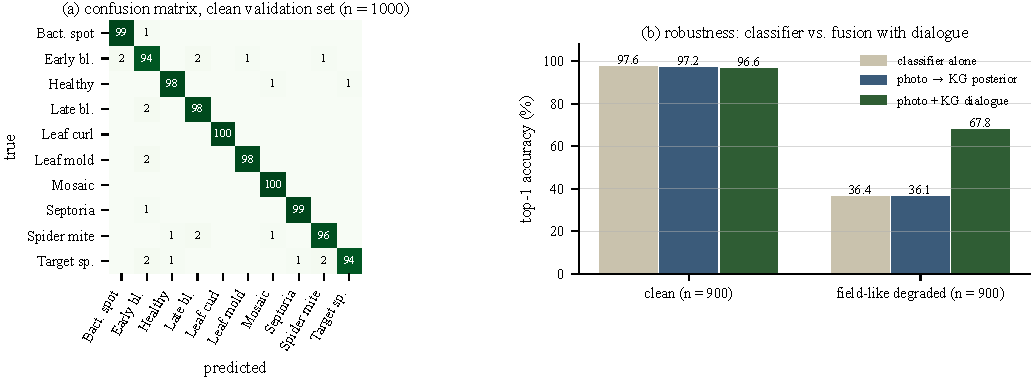
\includegraphics[width=\textwidth]{figures/vision.pdf}
  \caption{Leaf-photo classifier. (a) Confusion matrix on the clean validation set. (b) Top-1 accuracy on 900 disease images, clean and with field-like degradation, for the classifier alone, the KG posterior given only the photo, and the photo combined with the information-gain dialogue.}
  \label{fig:vision}
\end{figure*}

\subsection{Online learning}
To test whether feedback repairs an imperfect graph, the true KG generates 1,500 simulated consultations while the system starts from a corrupted copy: 15\% of symptom edges are set to 0.05 (knowledge gaps) and the rest are perturbed with Gaussian noise ($\sigma=0.25$). A simulated farmer describes two present symptoms, answers questions truthfully, confirms correct diagnoses and picks the correct disease for 70\% of wrong ones. Fig.~\ref{fig:learning} (five seeds) shows that the proposed rule raises accuracy from 81.2\% in the first 100 consultations to 93.6\% in the last 100 and reduces the mean absolute error of the 131 edge weights from 0.222 to 0.128. The prototype's rule ($\pm0.03$ on the predicted disease's edges after confirmation or rejection) reaches only 83.6\% and \emph{increases} the weight error to 0.239, because rejections punish edges of the wrong disease without teaching the right one; without learning accuracy stays near 79\%.

\begin{figure}[t]
  \centering
  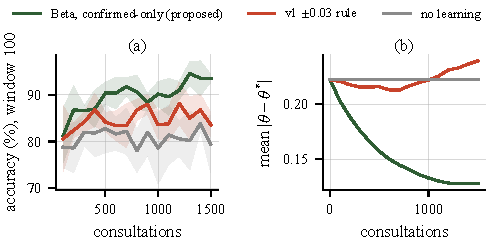
\includegraphics[width=\columnwidth]{figures/learning.pdf}
  \caption{Learning from feedback, starting from a corrupted KG (mean of five seeds; band: $\pm1$ s.d.). (a) Accuracy in windows of 100 consultations. (b) Mean absolute error of edge weights against the true graph.}
  \label{fig:learning}
\end{figure}

\subsection{Weather case study}
Fig.~\ref{fig:weather} shows the risk models on live weather for four districts on 13 October 2026. The Nilgiris (Ooty), at a three-day mean of 15.3\,$^\circ$C and 79\% RH, has five Hutton late-blight periods in the past week with another forecast (risk 1.0) and 96 hours above 85\% RH (leaf mold, 0.8). Krishnagiri, warm and dry, has 34 hot-dry hours (spider mite, 0.8), and Madurai five days above 33\,$^\circ$C (blossom-end rot, 0.8). Coimbatore shows only medium risks: its two Hutton periods are damped by a 26.3\,$^\circ$C mean temperature. These patterns are agronomically plausible but are not validated against observed outbreaks.

\begin{figure}[t]
  \centering
  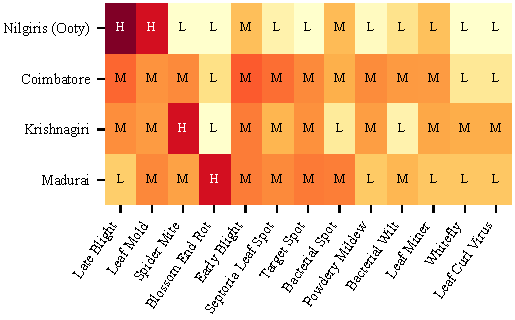
\includegraphics[width=\columnwidth]{figures/weather_risk.pdf}
  \caption{Weather-driven risk scores (colour) and levels (H/M/L) for four Tamil Nadu districts, computed from seven days of hourly weather on 13 October 2026.}
  \label{fig:weather}
\end{figure}

\subsection{Latency}
On a 12-thread laptop CPU without a GPU (Table~\ref{tab:latency}), concept matching takes 2.0\,ms, one inference step including the information-gain search 0.84\,ms, and a complete diagnosis request through the web API 3.7\,ms (median). Photo classification takes 7.1\,ms. The system therefore runs on commodity hardware, and the graph can be served from a small server.

\begin{table}[t]
  \caption{Latency on a laptop CPU (milliseconds)}
  \label{tab:latency}
  \centering
  \footnotesize
  \begin{tabular}{@{}lcc@{}}
    \toprule
    Operation & Median & 95th percentile \\
    \midrule
    Concept matching of one description & 2.01 & 2.58 \\
    Inference step (posterior + EIG search) & 0.84 & 0.87 \\
    Diagnosis API request (end to end) & 3.65 & 4.18 \\
    Leaf-photo classification (ONNX) & 7.12 & 8.09 \\
    \bottomrule
  \end{tabular}
\end{table}

% =====================================================================
\section{Discussion and Limitations}
\label{sec:limits}

The results support the central design choice: a curated, probabilistic KG that reasons over noisy evidence and asks targeted questions is robust where an image classifier alone is brittle, and it explains its answers in the farmer's language. Several limitations qualify these findings.
\begin{itemize}
  \item \emph{Evaluation data.} The test descriptions were written by the authors, and the simulated farmer answers according to the KG's own probabilities; the results therefore measure the reasoning pipeline, not field accuracy. A field study with real farmer descriptions and agronomist-confirmed diagnoses is the necessary next step.
  \item \emph{Knowledge.} Edge weights are expert estimates seeded from a dataset and extension guidance; Tamil lay-terms cover common usage but not all regional dialects. The learning loop and the curation queue are designed to correct both, but their effect in the field remains to be measured.
  \item \emph{Photo model.} The classifier was trained on laboratory images of nine diseases; its validation accuracy is optimistic, and the degradation study approximates, but does not replace, real field photographs.
  \item \emph{Weather models.} The Hutton criteria and TOM-CAST were developed for temperate climates and the remaining risk models are heuristics; none has yet been validated against outbreaks in Tamil Nadu. Community outbreak data shown in this paper are simulated.
  \item \emph{LLM front end and advice.} The Gemini speech front end was not evaluated quantitatively. Dosages are taken from the cited dataset or general guidance and must be checked against product labels and local recommendations.
\end{itemize}

% =====================================================================
\section{Conclusion}

Tomato Doctor combines a probabilistic knowledge graph, concept-level understanding of Tamil, English and Tanglish, Bayesian evidence fusion, cost-aware information-gain questioning, weather-driven priors and spray planning, and confirmation-driven learning. In our evaluation it raises top-1 accuracy from 63.5\% to 96.8\% over the fuzzy-matching prototype with about two questions, keeps confidently wrong answers near 1\%, recovers from degraded photographs through dialogue, and repairs a corrupted graph from farmer feedback. Future work will validate the system with farmers and agronomists in Tamil Nadu, calibrate the risk models against local outbreak records, extend the graph to further crops, and evaluate the speech front end on recorded farmer queries.

\section*{Acknowledgment}
The authors thank the farmers and agricultural extension staff who shared their vocabulary and experience. % edit as appropriate

% =====================================================================
\begin{thebibliography}{99}
\footnotesize

\bibitem{mohanty2016}
S.~P. Mohanty, D.~P. Hughes, and M.~Salath\'{e}, ``Using deep learning for image-based plant disease detection,'' \emph{Front. Plant Sci.}, vol.~7, Art. no.~1419, 2016, doi: 10.3389/fpls.2016.01419.

\bibitem{ferentinos2018}
K.~P. Ferentinos, ``Deep learning models for plant disease detection and diagnosis,'' \emph{Comput. Electron. Agric.}, vol.~145, pp.~311--318, 2018, doi: 10.1016/j.compag.2018.01.009.

\bibitem{barbedo2018}
J.~G.~A. Barbedo, ``Factors influencing the use of deep learning for plant disease recognition,'' \emph{Biosyst. Eng.}, vol.~172, pp.~84--91, 2018, doi: 10.1016/j.biosystemseng.2018.05.013.

\bibitem{hughes2015}
D.~P. Hughes and M.~Salath\'{e}, ``An open access repository of images on plant health to enable the development of mobile disease diagnostics,'' 2015, \emph{arXiv:1511.08060}.

\bibitem{heckerman1992}
D.~E. Heckerman, E.~J. Horvitz, and B.~N. Nathwani, ``Toward normative expert systems: Part~I. The Pathfinder project,'' \emph{Methods Inf. Med.}, vol.~31, no.~2, pp.~90--105, 1992.

\bibitem{shwe1991}
M.~A. Shwe \emph{et~al.}, ``Probabilistic diagnosis using a reformulation of the INTERNIST-1/QMR knowledge base. I. The probabilistic model and inference algorithms,'' \emph{Methods Inf. Med.}, vol.~30, no.~4, pp.~241--255, 1991.

\bibitem{lindley1956}
D.~V. Lindley, ``On a measure of the information provided by an experiment,'' \emph{Ann. Math. Statist.}, vol.~27, no.~4, pp.~986--1005, 1956.

\bibitem{hogan2021}
A.~Hogan \emph{et~al.}, ``Knowledge graphs,'' \emph{ACM Comput. Surv.}, vol.~54, no.~4, Art. no.~71, 2021.

\bibitem{chen2019agrikg}
Y.~Chen, J.~Kuang, D.~Cheng, J.~Zheng, M.~Gao, and A.~Zhou, ``AgriKG: An agricultural knowledge graph and its applications,'' in \emph{Database Systems for Advanced Applications (DASFAA 2019)}, Lecture Notes in Computer Science, vol.~11448. Cham, Switzerland: Springer, 2019.

\bibitem{jain2018farmchat}
M.~Jain, P.~Kumar, I.~Bhansali, Q.~V. Liao, K.~Truong, and S.~Patel, ``FarmChat: A conversational agent to answer farmer queries,'' \emph{Proc. ACM Interact. Mob. Wearable Ubiquitous Technol.}, vol.~2, no.~4, Art. no.~170, Dec. 2018, doi: 10.1145/3287048.

\bibitem{kakwani2020}
D.~Kakwani \emph{et~al.}, ``IndicNLPSuite: Monolingual corpora, evaluation benchmarks and pre-trained multilingual language models for Indian languages,'' in \emph{Findings of the Association for Computational Linguistics: EMNLP 2020}, 2020.

\bibitem{radford2023whisper}
A.~Radford, J.~W. Kim, T.~Xu, G.~Brockman, C.~McLeavey, and I.~Sutskever, ``Robust speech recognition via large-scale weak supervision,'' in \emph{Proc. Int. Conf. Mach. Learn. (ICML)}, 2023.

\bibitem{gemini2023}
Gemini Team, Google, ``Gemini: A family of highly capable multimodal models,'' 2023, \emph{arXiv:2312.11805}.

\bibitem{madden1978}
L.~Madden, S.~P. Pennypacker, and A.~A. MacNab, ``FAST, a forecast system for \emph{Alternaria solani} on tomato,'' \emph{Phytopathology}, vol.~68, pp.~1354--1358, 1978, doi: 10.1094/Phyto-68-1354.

\bibitem{frost2015}
K.~Frost, A.~Gevens, S.~Jordan, and R.~Groves, ``Web-based pest and disease forecasting tool for enhanced processing vegetable crop management: Update on carrot foliar disease forecasting component,'' in \emph{Proc. 2015 Wisconsin Crop Management Conf.}, vol.~54, 2015, pp.~83--85.

\bibitem{ahdb_hutton}
Agriculture and Horticulture Development Board (AHDB), ``Development and implementation of a new national warning system for potato late blight in Great Britain (Hutton Criteria).'' [Online]. Available: \url{https://potatoes.ahdb.org.uk/development-and-implementation-of-a-new-national-warning-system-for-potato-late-blight-in-great-britain-hutton-criteria}

\bibitem{jagtap2025}
S.~Jagtap, O.~Shinde, M.~Marade, R.~Sawant, N.~Sable, and P.~Mahalle, ``A comprehensive dataset of tomato plant diseases for national predictive analytics and crop health management,'' Mendeley Data, V1, 2025, doi: 10.17632/ztncd79yhk.1.

\bibitem{frac}
Fungicide Resistance Action Committee, ``FRAC Code List.'' [Online]. Available: \url{https://www.frac.info}

\bibitem{irac}
Insecticide Resistance Action Committee, ``IRAC Mode of Action Classification Scheme.'' [Online]. Available: \url{https://irac-online.org}

\bibitem{grapepath}
``Rains and fungicide sprays,'' Grape pathology extension. [Online]. Available: \url{https://ext.grapepathology.org/rains-and-fungicide-sprays}

\bibitem{awri2021}
The Australian Wine Research Institute, ``Agrochemical update: Using sulfur to protect vines, particularly under cool conditions,'' eBulletin, Oct. 2021. [Online]. Available: \url{https://www.awri.com.au/information_services/ebulletin/2021/10/13/agrochemical-update-october-2021-using-sulfur-to-protect-vines-particularly-under-cool-conditions/}

\bibitem{sparckjones1972}
K.~Sp\"{a}rck~Jones, ``A statistical interpretation of term specificity and its application in retrieval,'' \emph{J. Documentation}, vol.~28, no.~1, pp.~11--21, 1972.

\bibitem{openmeteo}
P.~Zippenfenig, ``Open-Meteo.com weather API,'' Zenodo, 2023, doi: 10.5281/zenodo.7970649.

\bibitem{agvic_wind}
Agriculture Victoria, ``A guide to estimating wind speed.'' [Online]. Available: \url{https://agriculture.vic.gov.au/farm-management/chemicals/spraying-agricultural-chemicals/managing-spray-drift/a-guide-to-estimating-wind-speed}

\bibitem{neo4j}
Neo4j, Inc., ``Neo4j graph database.'' [Online]. Available: \url{https://neo4j.com}

\bibitem{howard2019}
A.~Howard \emph{et~al.}, ``Searching for MobileNetV3,'' in \emph{Proc. IEEE/CVF Int. Conf. Comput. Vis. (ICCV)}, 2019, pp.~1314--1324.

\bibitem{loshchilov2019}
I.~Loshchilov and F.~Hutter, ``Decoupled weight decay regularization,'' in \emph{Proc. Int. Conf. Learn. Represent. (ICLR)}, 2019.

\bibitem{szegedy2016}
C.~Szegedy, V.~Vanhoucke, S.~Ioffe, J.~Shlens, and Z.~Wojna, ``Rethinking the Inception architecture for computer vision,'' in \emph{Proc. IEEE Conf. Comput. Vis. Pattern Recognit. (CVPR)}, 2016, pp.~2818--2826.

\bibitem{guo2017}
C.~Guo, G.~Pleiss, Y.~Sun, and K.~Q. Weinberger, ``On calibration of modern neural networks,'' in \emph{Proc. Int. Conf. Mach. Learn. (ICML)}, 2017, pp.~1321--1330.

\bibitem{efron1993}
B.~Efron and R.~J. Tibshirani, \emph{An Introduction to the Bootstrap}. New York, NY, USA: Chapman \& Hall, 1993.

\end{thebibliography}

\end{document}
